\documentclass[9pt]{extarticle}
\usepackage[a4paper,margin=1in]{geometry}
\usepackage[T1]{fontenc}
\usepackage{mathptmx}
\usepackage[expansion=false]{microtype}
\DeclareUnicodeCharacter{2190}{\ensuremath{\leftarrow}}
\usepackage{graphicx}
\usepackage{booktabs}
\usepackage{array}
\usepackage{longtable}
\usepackage{multirow}
\usepackage[font=small,labelfont=bf,skip=3pt]{caption}
\usepackage{subcaption}
\usepackage{enumitem}
\usepackage{titlesec}
\setlist{nosep,leftmargin=1.2em}
\titlespacing*{\section}{0pt}{8pt}{3pt}
\titlespacing*{\subsection}{0pt}{6pt}{2pt}
\setlength{\parskip}{2pt}
\setlength{\textfloatsep}{8pt}
\setlength{\floatsep}{6pt}
\setlength{\intextsep}{6pt}
\newcommand{\Q}[1]{\textbf{\emph{Q: #1}}}
\newcommand{\run}[1]{\textsf{#1}}

\begin{document}

\begin{center}
{\large\textbf{Lab 1 -- Introduction to Deep Learning: building, training and judging a feed-forward network}}\\[3pt]
\textbf{Group 18} -- Andrea De Vito (s349609), Davide Di Pasquale (s348493),\\ Gabriele Audo (s349636), Gabriele Loguercio Polosa (s348818)
\end{center}

\noindent\textbf{Setup and conventions.} All experiments are in \texttt{group18\_lab1.ipynb}; each run has a Markdown header with its logbook ID and the run it starts from (e.g.\ \run{R2 (←R1L)}). The logbook (Appendix A) has \textbf{27 runs}: 10 in Task 2, 2 in Task 4, 10 in Task 5 and 5 in Task 6, two more than the $\sim$25 of the lab text (\run{S2-lr0.01} and \run{D2}, both redundant in hindsight; see the final reflection). Every choice is made on the validation set; a test set is used once per model we decided to report. Seeds are fixed (initial weights and batch order are identical across runs) and the final notebook was executed top to bottom on CPU on one machine. Our selection metric is the validation macro-F1 (justified in Task 4); we also report missed attacks (attack flows predicted Benign) and false alarms (Benign flows predicted as an attack). The ``best epoch'' is the one whose weights are restored: early stopping counts an improvement only above $10^{-4}$, so it can differ from the epoch of the raw minimum of the validation loss (e.g.\ \run{R1L}: best epoch 99 at 0.0273, raw minimum 0.0272 at epoch 100).

%==========================================================
\section{Task 1 -- Preprocessing}

\textbf{Inspection.} The CSV has 31,507 flows, 16 features and 4 classes: Benign 20,000 (63.48\%), DoS Hulk 5,000 (15.87\%), PortScan 5,000 (15.87\%), Brute Force 1,507 (4.78\%). Brute Force is the rare class. We found 20 missing values (Flow Bytes/s), 7 infinite values in Flow Bytes/s and 27 in Flow Packets/s, 2 rows with negative durations (Flow Duration $=-1$, which also makes the derived rates negative), 2,111 duplicated rows, and two pairs of identical columns (Fwd PSH Flags = SYN Flag Count, Subflow Fwd Packets = Total Fwd Packets). We keep both columns of each pair: for a neural network a duplicated input adds no information but does no harm.

\textbf{Cleaning.} We applied four steps, in this order (Table~\ref{tab:clean}). (a) NaN and $\pm\infty$: the affected rate features are $x/0$ or $0/0$ over a zero-length flow, so the value cannot be recovered; dropping 27 rows (0.09\%) is cheaper and safer than inventing a rate. (b) Negative durations are physically impossible: 2 rows dropped. (c) Exact duplicates (features \emph{and} label) are dropped \emph{before} the split, otherwise identical copies could end up in both training and test and reward memorisation. (d) After (c), 7 feature vectors still appear once as Benign and once as DoS Hulk: no model can classify both, so all 14 copies are dropped.

\begin{table}[h]
\centering\small
\begin{tabular}{lrrrrrr}
\toprule
class & raw & after NaN/inf & after negatives & after duplicates & clean & \% lost \\
\midrule
Benign & 20,000 & 19,992 & 19,990 & 19,240 & 19,233 & 3.8 \\
Brute Force & 1,507 & 1,507 & 1,507 & 1,427 & 1,427 & 5.3 \\
DoS Hulk & 5,000 & 4,982 & 4,982 & 3,868 & 3,861 & 22.8 \\
PortScan & 5,000 & 4,999 & 4,999 & 4,849 & 4,849 & 3.0 \\
\textbf{total} & 31,507 & 31,480 & 31,478 & 29,384 & 29,370 & 6.8 \\
\bottomrule
\end{tabular}
\caption{Per-class counts after each cleaning step. De-duplication hits DoS Hulk much harder than the other classes.}
\label{tab:clean}
\end{table}

\Q{How many samples before and after cleaning?} $\rightarrow$ 31,507 before, \textbf{29,370} after (6.8\% removed), almost all of it duplicates. The losses are uneven: DoS Hulk loses 22.8\% (repeated identical requests), the other classes 3--5\%.

\textbf{Split.} 70/15/15, stratified, fixed seed: 20,559 / 4,405 / 4,406 flows. With 15\%, Brute Force still has 214 flows in validation and test (one flow $\approx$ 0.5 points of recall).

\Q{Should the split be stratified? Where did you fit the scaler, and what goes wrong if you fit it on all the data?} $\rightarrow$ Yes: with Brute Force under 5\%, a random split could give validation and test noticeably fewer Brute Force flows, and the per-class metrics would depend on the luck of the split. With stratification the class shares differ by at most 0.02 points across the three partitions (Brute Force 4.86\% in all three). The scaler is fitted on the training set only and applied unchanged to validation and test. Fitting it on all the data would put their mean and standard deviation into the preprocessing (leakage), so the evaluation would be on data that already shaped the model, and the scores would be optimistic.

\textbf{Scaling.} The features are strongly right-skewed (skew up to 63.44, maximum $z$ up to 84.95) and span from 0/1 flags to $2.07\cdot10^9$ (Flow Bytes/s).

\Q{Which scaling did you pick and why? How did the outliers inform the choice?} $\rightarrow$ \textbf{StandardScaler, fitted on the training set}, and we keep the outliers. Three observations drove the choice. (i) The outliers are class-typical, not errors: 78.1--85.9\% of the DoS Hulk flows are beyond the boxplot whiskers in six features, and 54.4\% of PortScan flows in Destination Port; removing them would remove part of the attack classes. (ii) Min-Max divides by the full range, so one extreme value squeezes the central half of the data: the IQR of Total Fwd Packets would be 0.0013 of the scale instead of 0.1084 with standard scaling (85$\times$ narrower). (iii) Standard scaling has a known limit: it rescales the tails but does not remove them. The bulk of Flow Bytes/s stays near zero (96.94\% of the flows within $|z|<0.1$) and validation contains a Benign flow with 18,605 forward packets against a training maximum of 3,141 ($|z| = 504.0$). A $\log(1+x)$ transform before the scaler fixes both (near-zero share 8.75\%, maximum $|z|$ 8.53 on training); we kept it as a hypothesis and tested it as one change in Task 2 (\run{R1L}), where it was adopted. Destination Port is treated as numeric as required; its profile already showed the problem of Task 3: in the training set Brute Force and DoS Hulk use only port 80, PortScan 967 ports and Benign 2,595 (10.7\% on port 80).

%==========================================================
\section{Task 2 -- Your first network}

\subsection*{2A -- A minimal working classifier}
\textbf{Choices.} One hidden layer of 64 ReLU units (1,348 parameters), cross-entropy, AdamW (lr $5\cdot10^{-4}$, default weight decay 0.01), batch 64, at most 100 epochs, early stopping on the validation loss (patience 10, minimum improvement $10^{-4}$) with the weights of the best epoch restored. To read the curves we use two reference levels: $\ln 4 = 1.386$ (a network that gives each class the same probability) and 0.988 (a network that only learned the class frequencies). The trivial ``always Benign'' accuracy on validation is 0.6549.

\textbf{Prediction (\run{R1}).} From Task 1 we expected Brute Force to be the hardest class (rarest, and inside the bulk of the data, without the extreme values of DoS Hulk or the many ports of PortScan), failing through missed detections predicted as Benign, and DoS Hulk and PortScan to be the easiest.

\begin{figure}[h]
\centering
\begin{subfigure}{0.49\linewidth}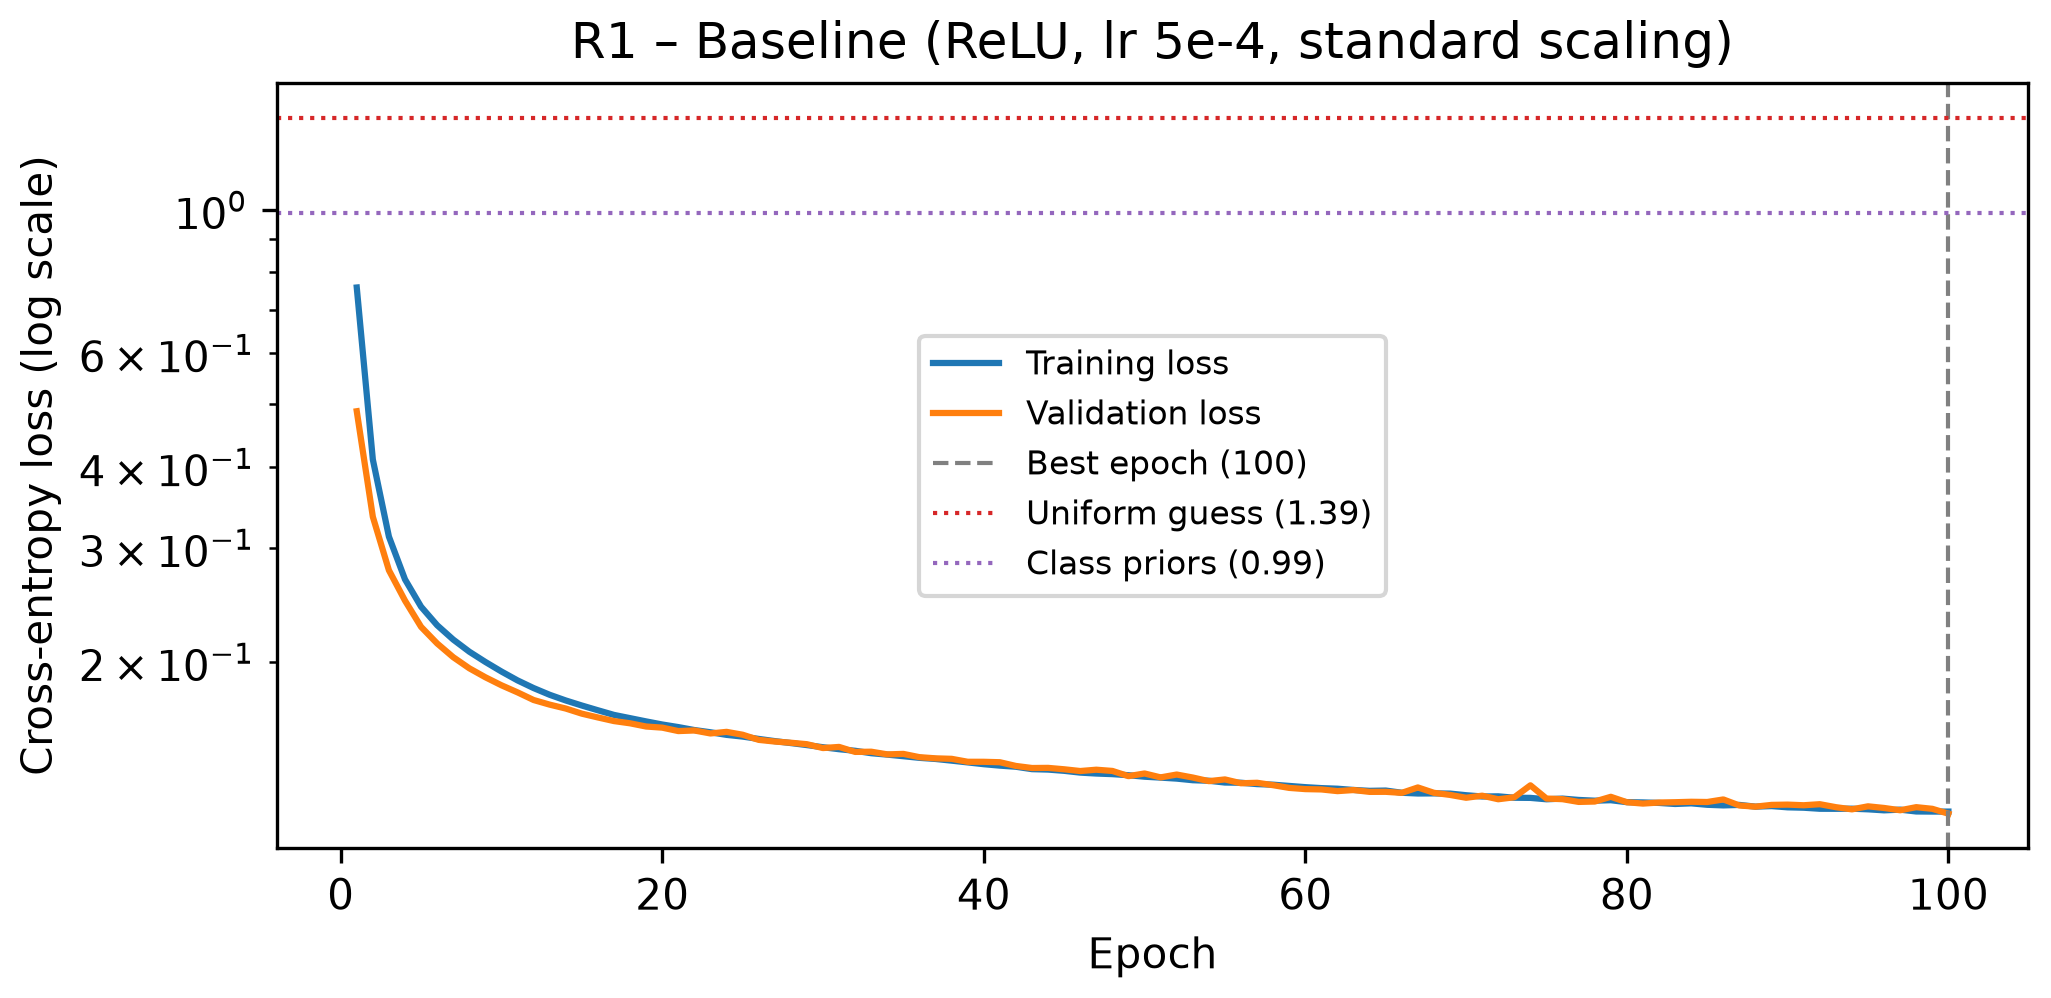
\includegraphics[width=\linewidth]{figures/R1_loss.png}\caption{\run{R1}: training and validation loss.}\end{subfigure}\hfill
\begin{subfigure}{0.49\linewidth}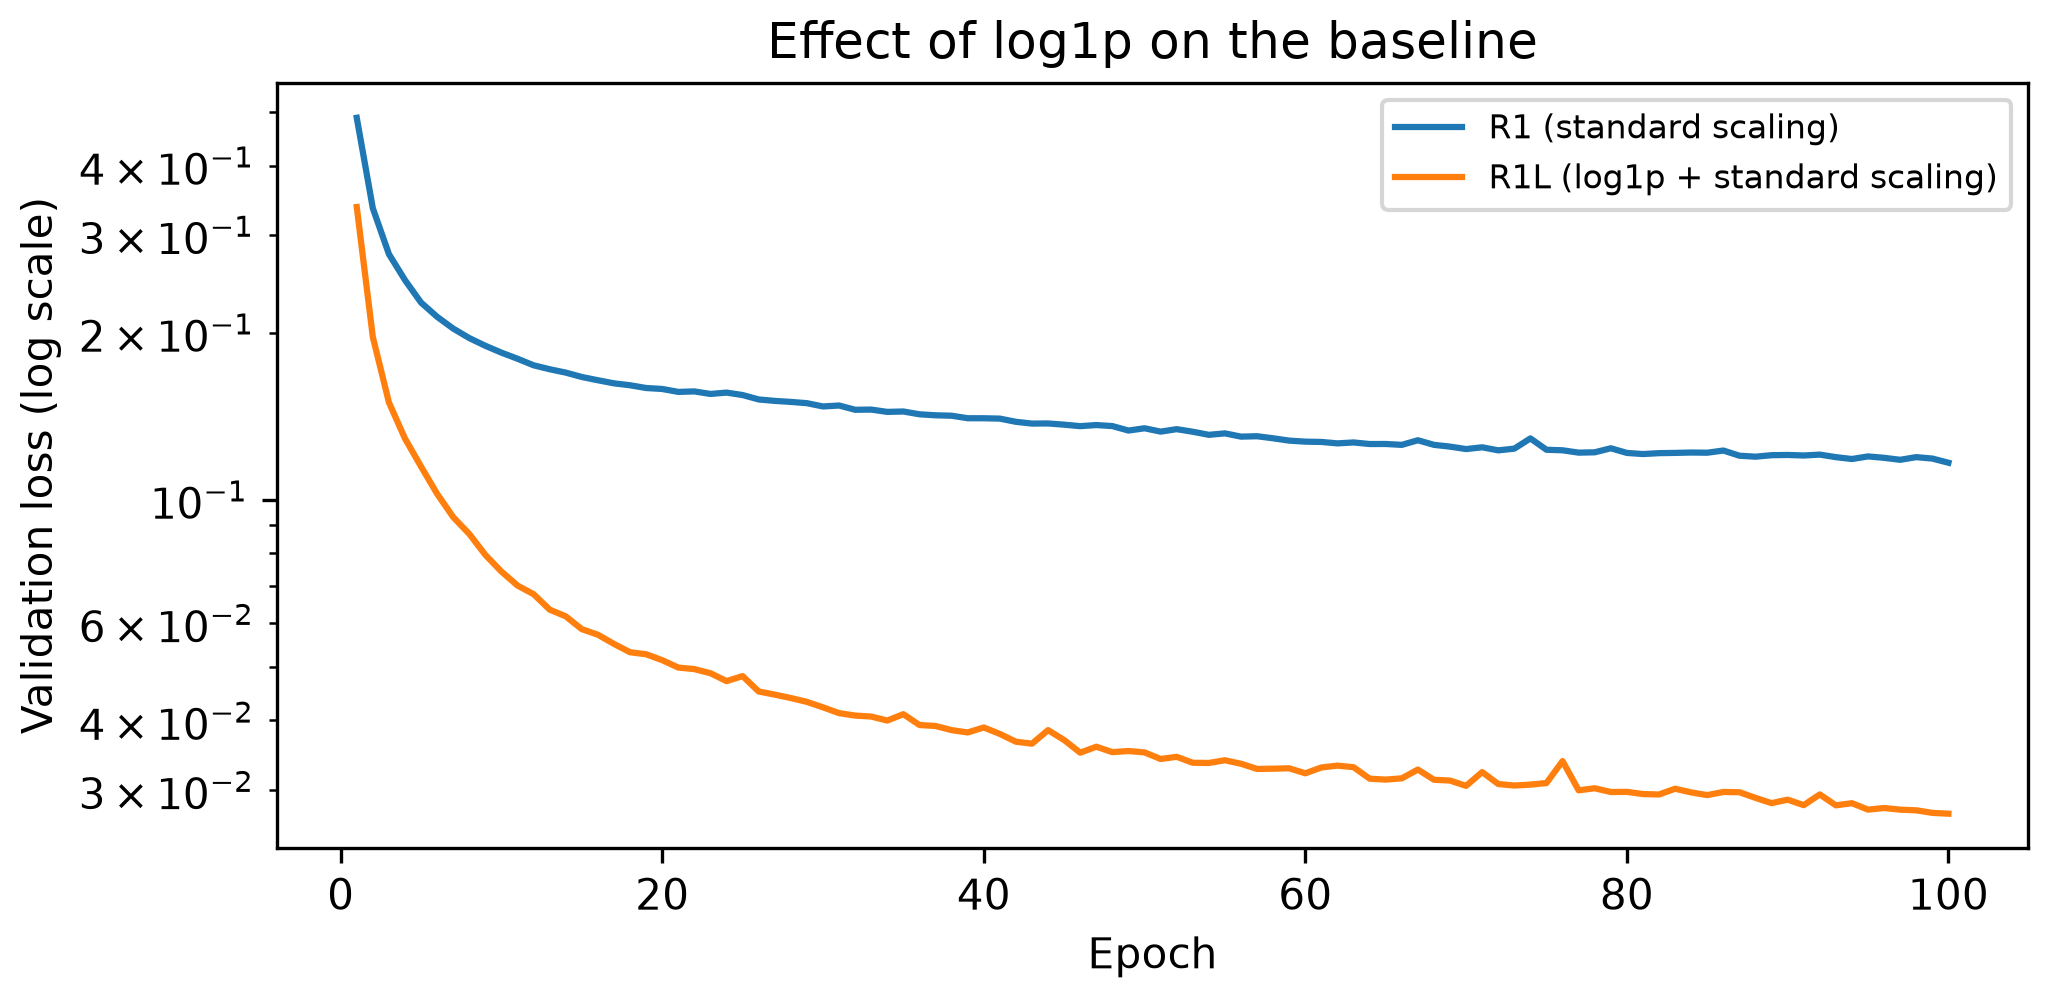
\includegraphics[width=\linewidth]{figures/R1_vs_R1L_val_loss.png}\caption{Validation loss of \run{R1} and \run{R1L}.}\end{subfigure}
\caption{The baseline is still improving at the 100-epoch cap (a). Adding $\log(1+x)$ before the scaler (b) lowers the validation loss at every epoch: 0.0742 vs 0.1841 at epoch 10, minimum 0.0272 vs 0.1166.}
\label{fig:r1}
\end{figure}

\Q{How do you pick the ``best'' model across epochs? Do the curves converge?} $\rightarrow$ We keep the epoch with the lowest validation loss. We prefer the loss to the validation macro-F1 because it uses the predicted probabilities and changes smoothly, while macro-F1 jumps only when a prediction flips, which is noisy on 214 Brute Force flows; the price is that we do not select directly on the metric we report. The curves do \textbf{not} converge within 100 epochs: the best epoch of \run{R1} is the last one (Fig.~\ref{fig:r1}a). Training and validation stay close; at epoch 1 the training loss is even higher (0.7580 vs 0.4880) because it is averaged while the weights change, whereas the validation loss is computed at the end of the epoch.

\Q{Do your hardest-class predictions hold up?} $\rightarrow$ Only in part (\run{R1}: accuracy 0.9587, macro-F1 0.9365; Table~\ref{tab:r1}). Brute Force has the lowest precision (0.824) and F1 (0.880), but its recall is 0.944, and its problem is false positives: 43 Benign flows predicted as Brute Force against 12 misclassified Brute Force flows (10 predicted as PortScan, only 2 as Benign). All 43 are on port 80: 13.8\% of the 311 Benign port-80 validation flows are flagged, 0.0\% of the 2,574 Benign flows on other ports. Our ``easy'' classes were wrong: PortScan and DoS Hulk have the lowest recalls (0.928 and 0.934; 50 and 38 flows predicted Benign). With standard scaling alone their distinguishing features sit in the squeezed bulk, which motivated the next run.

\begin{table}[h]
\centering\small
\begin{tabular}{lrcccccc}
\toprule
 & & \multicolumn{3}{c}{\run{R1}} & \multicolumn{3}{c}{\run{R1L}} \\
class & support & precision & recall & F1 & precision & recall & F1 \\
\midrule
Benign & 2,885 & 0.969 & 0.972 & 0.971 & 0.998 & 0.993 & 0.996 \\
Brute Force & 214 & 0.824 & 0.944 & 0.880 & 0.939 & 1.000 & 0.968 \\
DoS Hulk & 579 & 0.989 & 0.934 & 0.961 & 0.985 & 0.993 & 0.989 \\
PortScan & 727 & 0.940 & 0.928 & 0.934 & 1.000 & 0.994 & 0.997 \\
\midrule
accuracy / macro-F1 & 4,405 & \multicolumn{3}{c}{0.9587 / 0.9365} & \multicolumn{3}{c}{0.9936 / 0.9875} \\
\bottomrule
\end{tabular}
\caption{Validation classification reports of \run{R1} (standard scaling) and \run{R1L} ($\log(1+x)$ + standard scaling).}
\label{tab:r1}
\end{table}

\textbf{\run{R1L (←R1)}: $\log(1+x)$ before the scaler.} We fixed the rule beforehand: adopt it only if macro-F1 rises by at least 0.01 and no class loses more than 0.02 of recall. Macro-F1 rose to 0.9875 (+0.0510) and the errors fell from 182 to 28. We had predicted the gain on Brute Force precision (0.824 $\rightarrow$ 0.939, Benign port-80 flows flagged 13.8\% $\rightarrow$ 4.5\%), but the largest gains came where we expected none: DoS Hulk recall 0.934 $\rightarrow$ 0.993 and PortScan 0.928 $\rightarrow$ 0.994. Being ``extreme'' in raw scale did not make these classes easy; un-squeezing the bulk did. $\log(1+x)$ is used for the rest of the lab.

\subsection*{2B -- Why the fundamentals matter}
\run{S2} and \run{S3} change one fundamental of \run{R1L}. \run{S1} removes the scaling altogether: this is one change from \run{R1} (no StandardScaler) but two from \run{R1L} (no $\log(1+x)$ either), so its parent in the logbook is \run{R1}; \run{R1L} is shown as the common reference (Fig.~\ref{fig:fund}, Table~\ref{tab:fund}). Against its parent, \run{S1} takes the macro-F1 from 0.9365 to 0.6943.

\begin{figure}[h]
\centering
\begin{subfigure}{0.49\linewidth}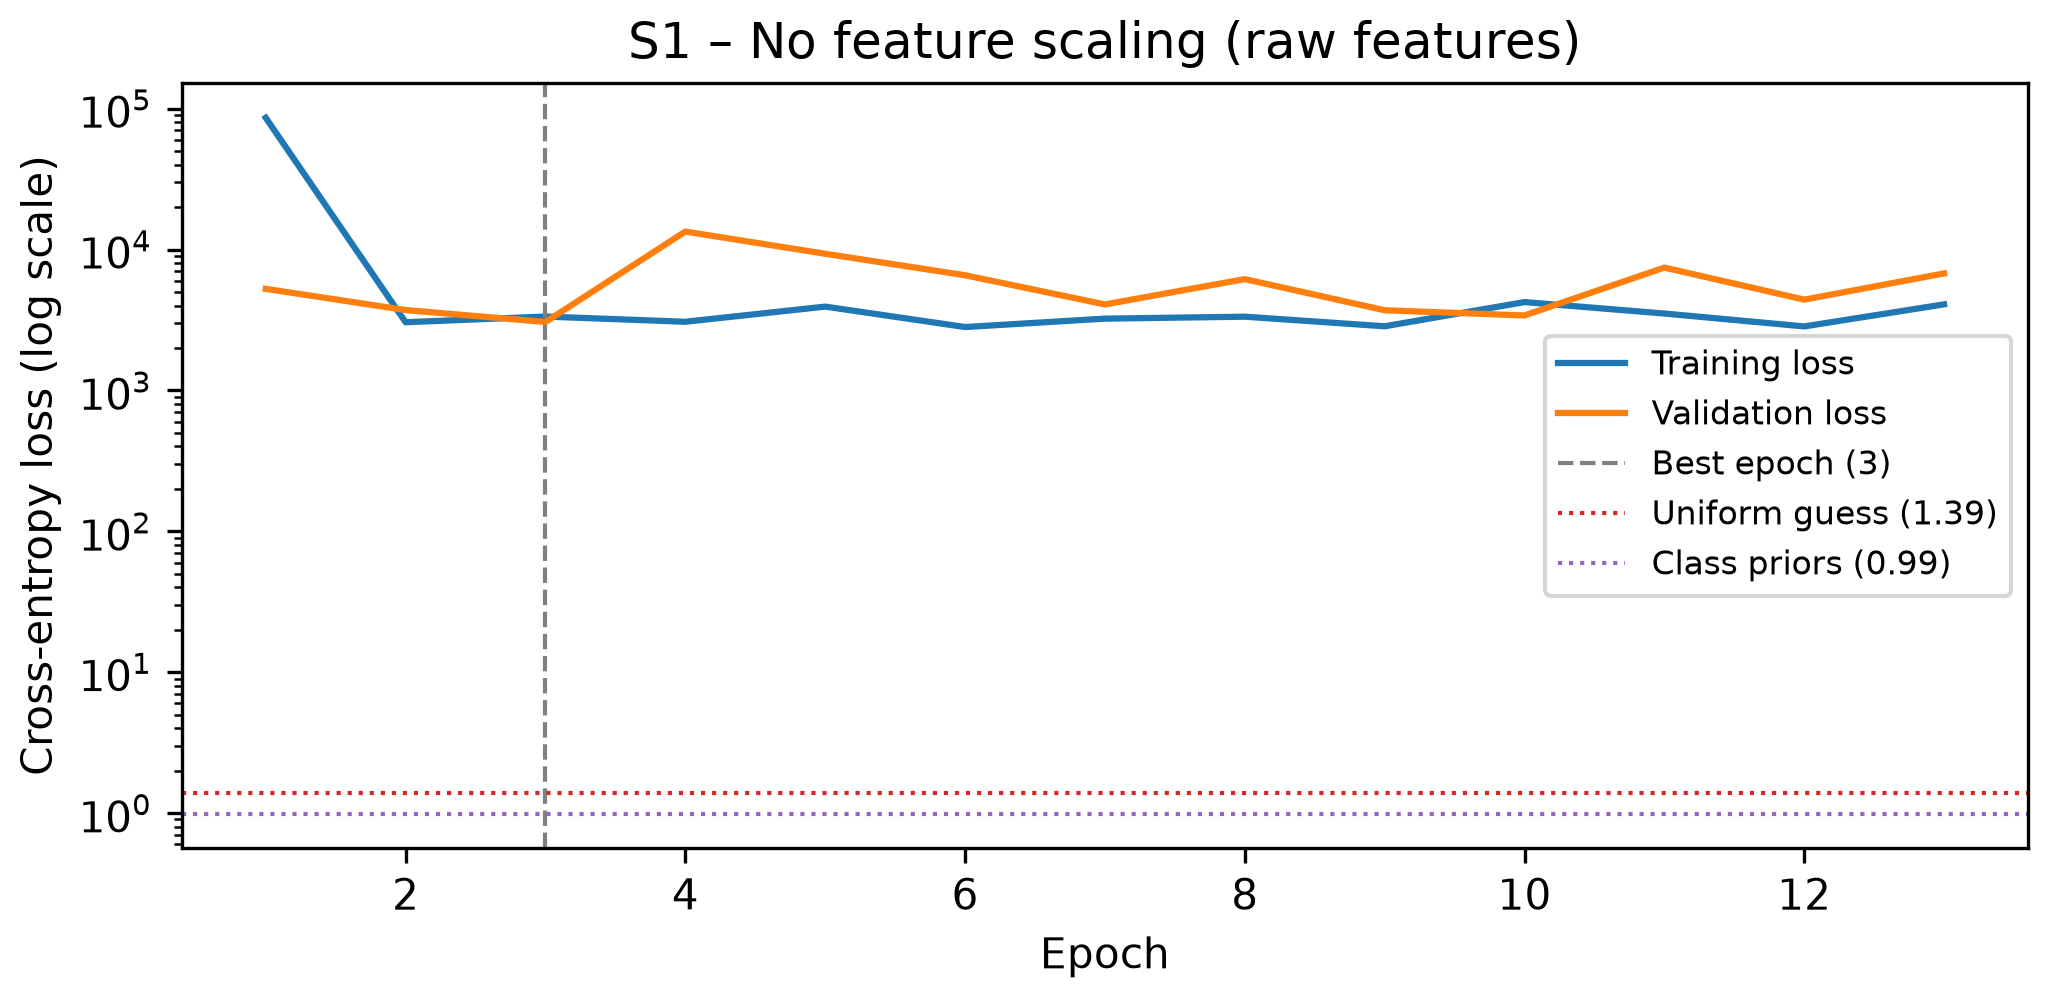
\includegraphics[width=\linewidth]{figures/S1_loss.png}\caption{\run{S1}: raw features.}\end{subfigure}\hfill
\begin{subfigure}{0.49\linewidth}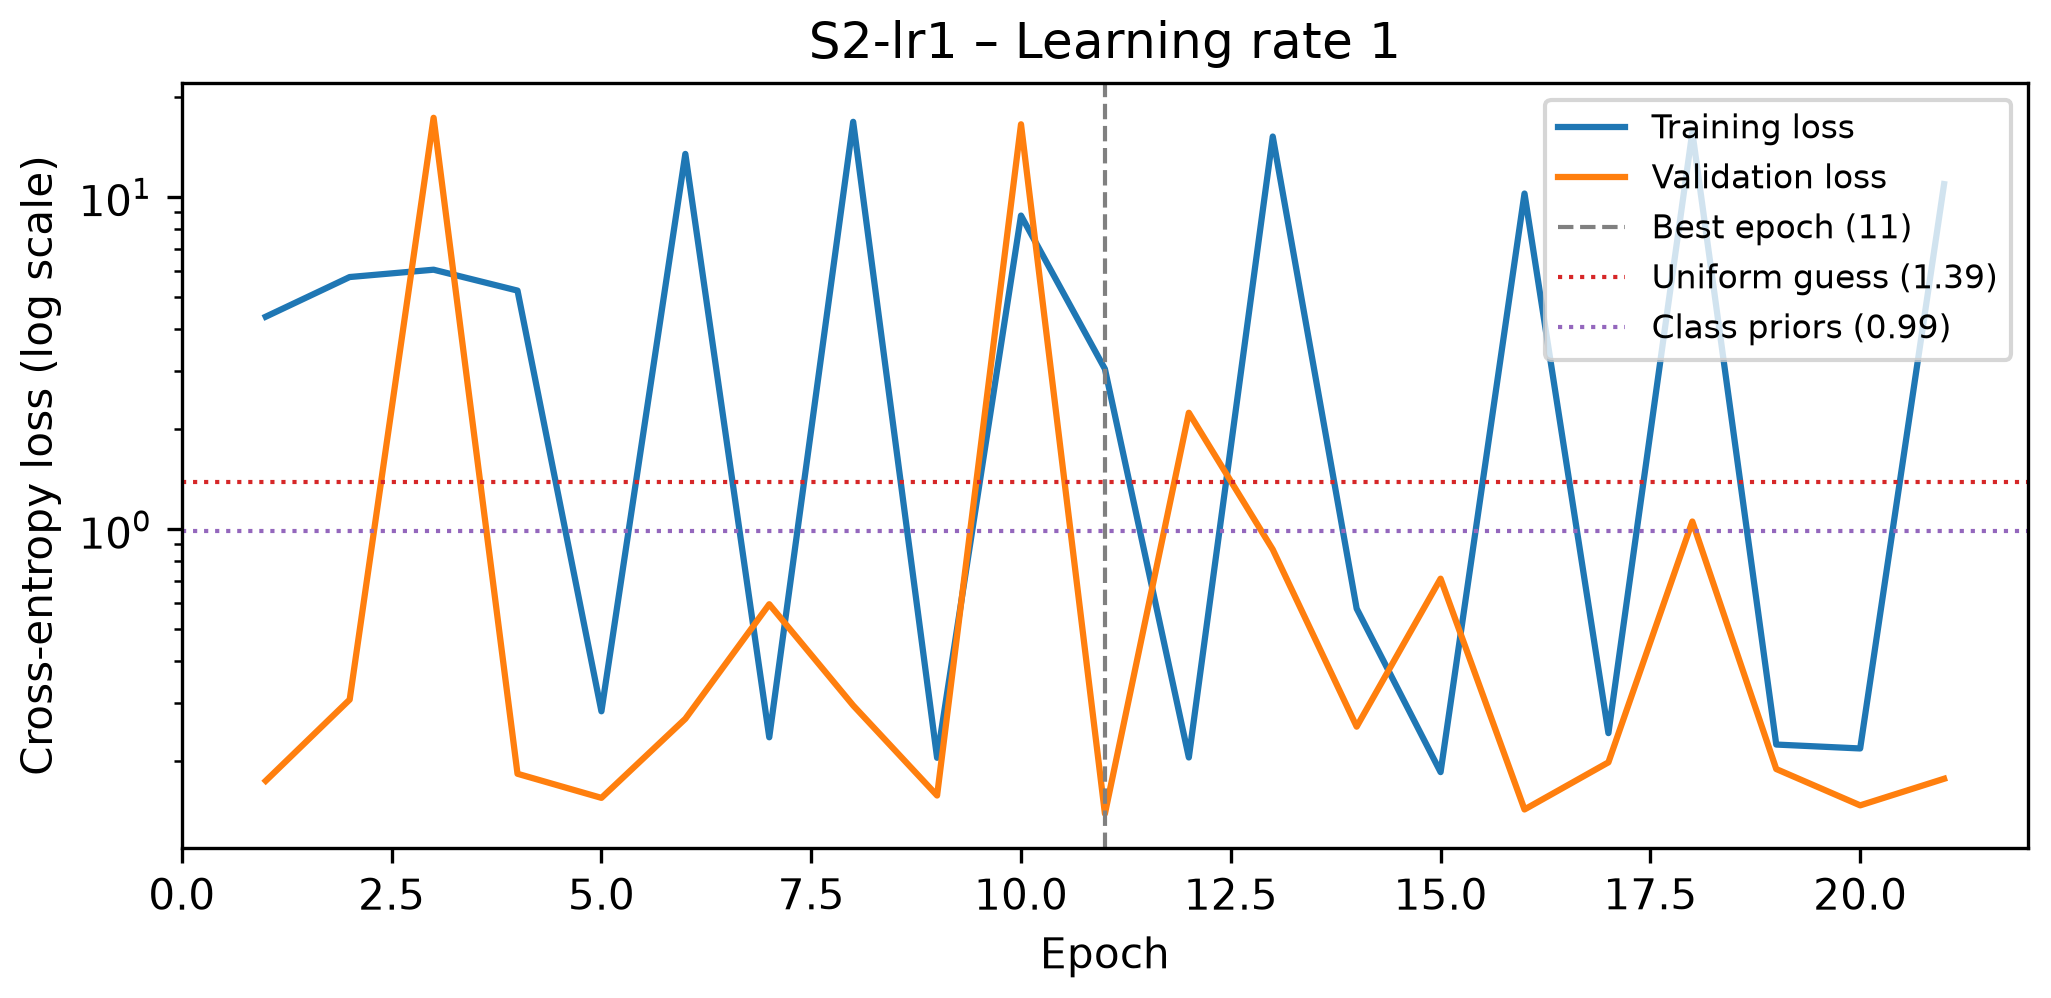
\includegraphics[width=\linewidth]{figures/S2-lr1_loss.png}\caption{\run{S2}: lr = 1.}\end{subfigure}\\[2pt]
\begin{subfigure}{0.49\linewidth}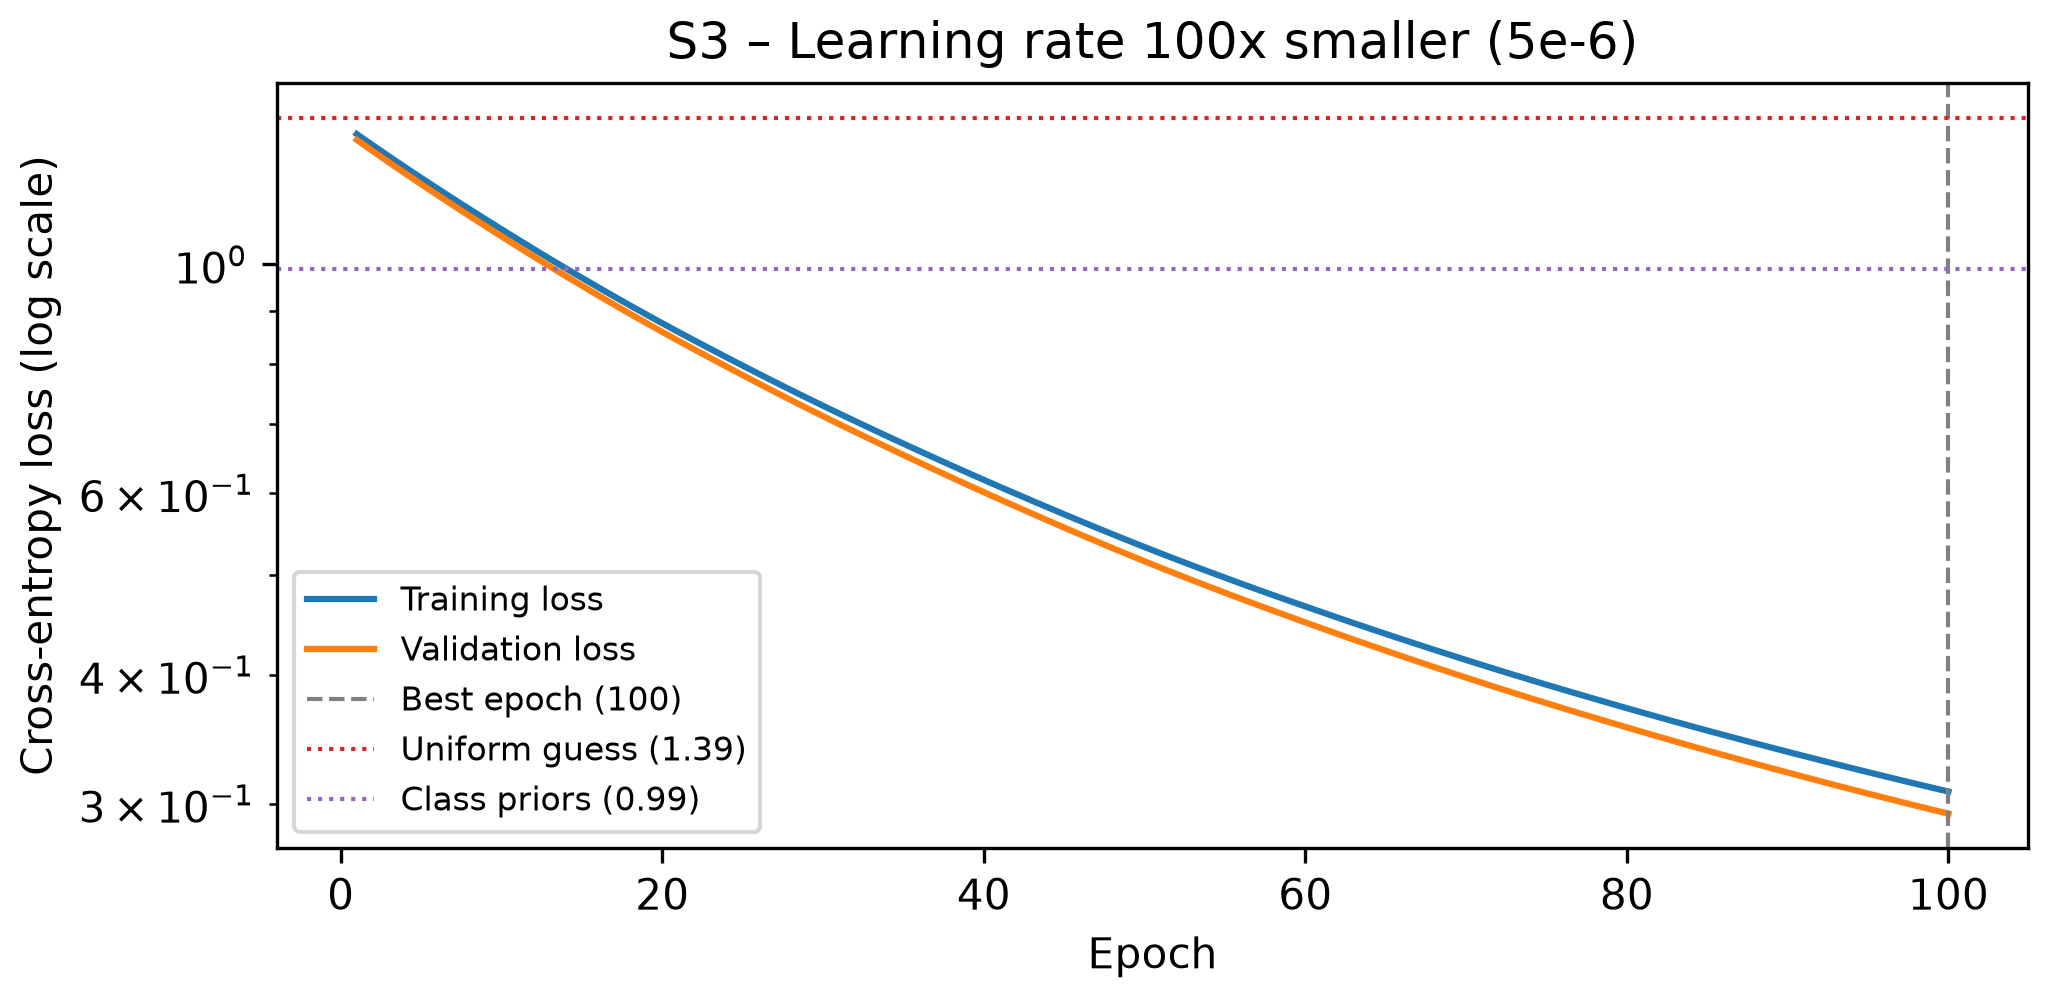
\includegraphics[width=\linewidth]{figures/S3_loss.png}\caption{\run{S3}: lr = $5\cdot10^{-6}$.}\end{subfigure}\hfill
\begin{subfigure}{0.49\linewidth}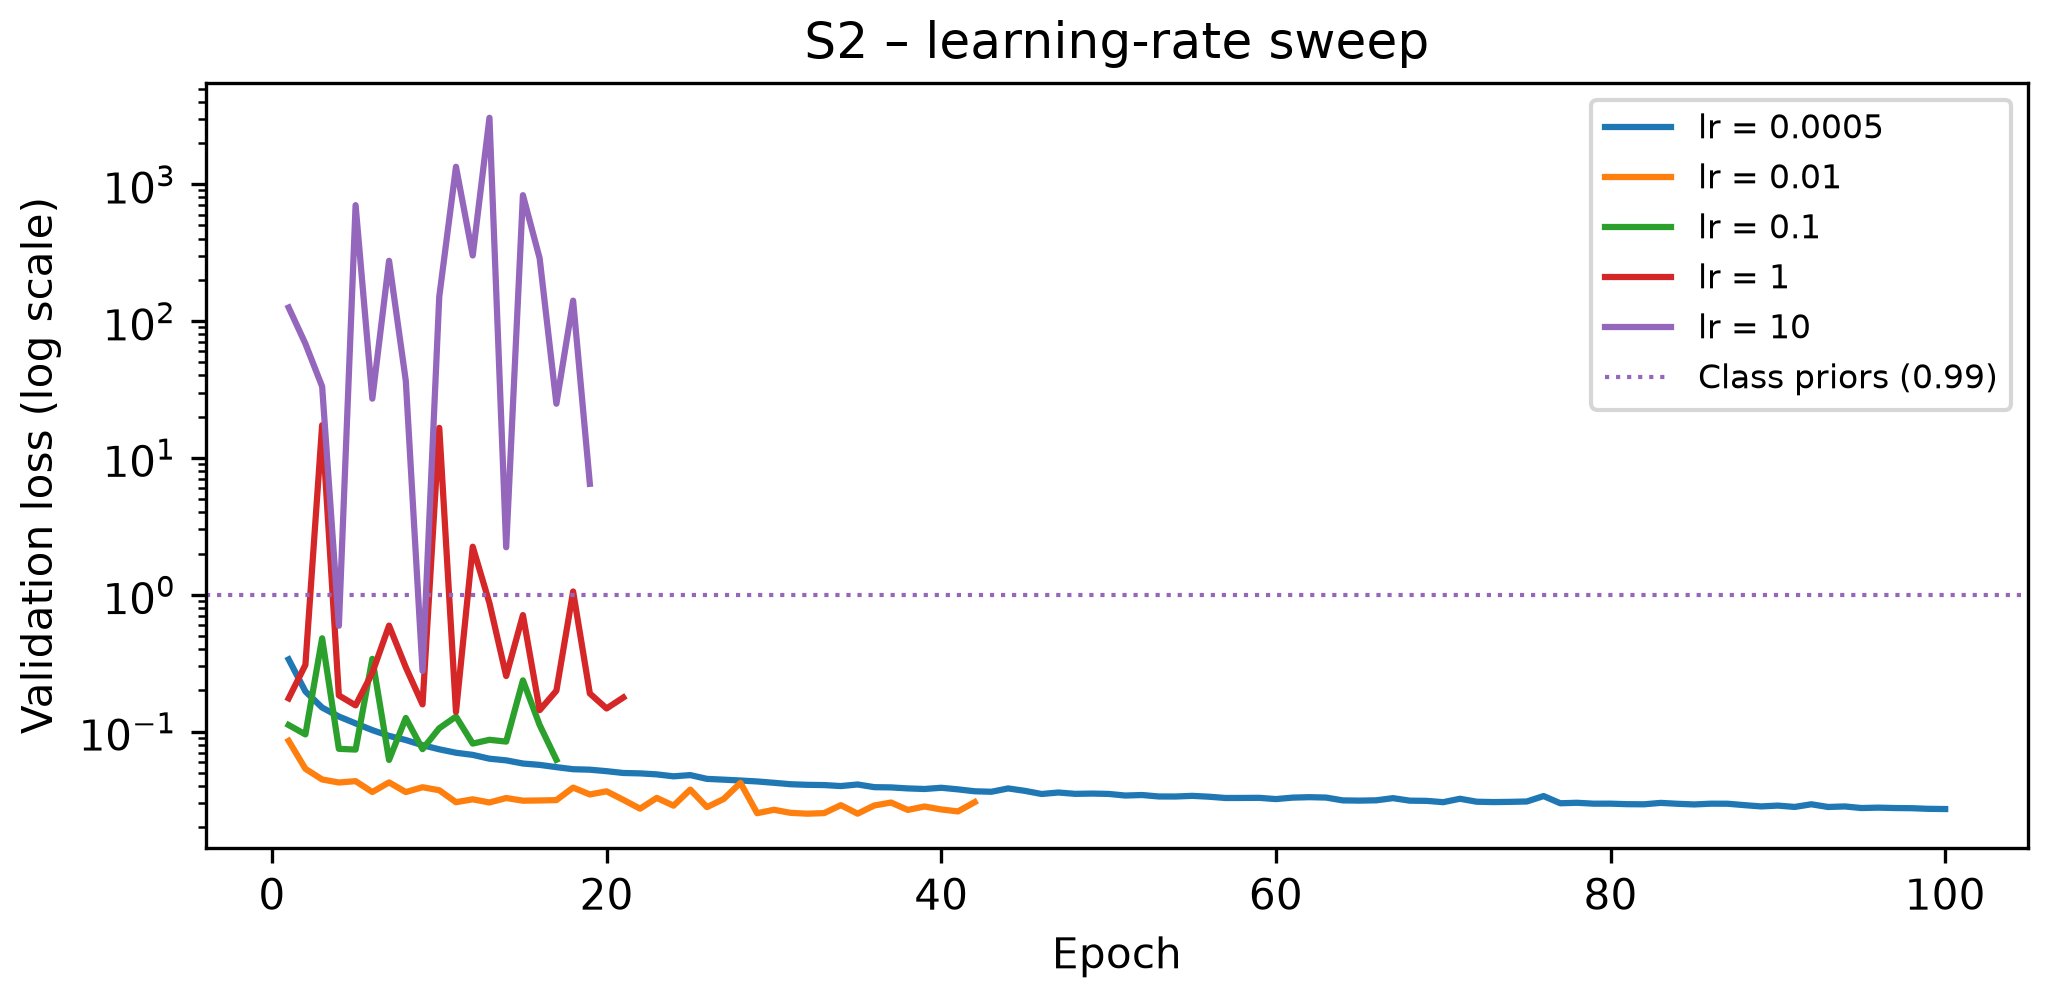
\includegraphics[width=\linewidth]{figures/S2_lr_sweep_val_loss.png}\caption{The S2 sweep: validation loss for each lr.}\end{subfigure}
\caption{Three failure modes (log scale; dotted lines: $\ln 4$ and class priors). (a) The loss stays three orders of magnitude above $\ln 4$ for the whole run. (b) The loss jumps by two orders of magnitude from one epoch to the next. (c) A smooth curve, train $\approx$ val, still falling at the last epoch. (d) The spikes grow with the lr, yet each run has a few low epochs that early stopping can pick.}
\label{fig:fund}
\end{figure}

\begin{table}[h]
\centering\small
\begin{tabular}{lrrrr}
\toprule
 & \run{R1L} & \run{S1} (raw) & \run{S2} (lr 1) & \run{S3} (lr $5\cdot10^{-6}$) \\
\midrule
macro-F1 (val) & 0.9875 & 0.6943 & 0.9036 & 0.9128 \\
first-epoch train loss & 0.6472 & 86142.1984 & 4.3650 & 1.3367 \\
min val loss & 0.0272 & 3058.5143 & 0.1393 & 0.2934 \\
val roughness (mean $|\Delta \ln$ loss$|$ per epoch) & 0.0361 & 0.4963 & 1.6570 & 0.0152 \\
val $-$ train at best epoch & $-0.0022$ & $-285.5191$ & $-2.8986$ & $-0.0149$ \\
val slope, last 10 epochs (\%/epoch) & $-0.5653$ & 12.1302 & 2.7399 & $-0.8773$ \\
best / last epoch & 99 / 100 & 3 / 13 & 11 / 21 & 100 / 100 \\
\bottomrule
\end{tabular}
\caption{The three variants of Task 2B against \run{R1L}. The ``roughness'' measures how much the validation loss jumps between consecutive epochs.}
\label{tab:fund}
\end{table}

\textbf{\run{S1} -- no scaling. Failure mode: badly conditioned inputs.} \emph{Prediction:} first-epoch loss between $10^3$ and $10^6$, a jagged curve and no NaN. \emph{Result:} right. The untrained network already has a loss of $1.373\cdot10^6$ (mean $|$logit$|$ $1.181\cdot10^6$, against 1.354 and 0.1797 with scaled inputs). The features with the largest values dominate the hidden pre-activations, the logits are huge and the softmax is saturated, so each mistake costs a loss of the order of its logit margin. AdamW moves every weight by about lr per step: on a feature of order $10^7$ this changes the logits by thousands, on a 0/1 flag almost nothing, and no single learning rate fits both. The loss stays around $3\cdot10^3$ for the whole run and Brute Force is never detected (recall 0.000, macro-F1 0.6943). We had also expected the loss might settle on the class-priors line; it never came close.

\textbf{\run{S2} -- learning rate too high. Failure mode: overshoot.} \Q{How high are you expecting the too-high LR to be?} $\rightarrow$ Around 1 (range 0.3--3, about $2000\times$ the baseline): Adam moves each weight by about lr, and with 16 standardised inputs one step can change a pre-activation by up to $\sim16\cdot$lr$\cdot|z|$. We swept lr = $10^{-2}$, $10^{-1}$, 1, 10 (\run{S2-lr0.01}, \run{S2-lr0.1}, \run{S2-lr1}, \run{S2-lr10}) with a criterion fixed beforehand: ``broken'' if the minimum validation loss exceeds 0.31 or a NaN appears. The shape confirmed the prediction: from lr = 1 the first-epoch training loss is above $\ln 4$ (4.3650; 388.1683 at lr = 10) and the validation loss jumps to 16.5687 at epoch 10 before coming back (Fig.~\ref{fig:fund}b). The criterion, however, was met by no lr (lr = 10 reaches 0.2775): early stopping restores the luckiest epoch of a jagged curve, so the minimum hides the breakdown. The roughness shows it clearly (Fig.~\ref{fig:fund}d; 0.0361 $\rightarrow$ 0.1289 $\rightarrow$ 0.723 $\rightarrow$ 1.657 $\rightarrow$ 3.2596). In hindsight \run{S2-lr0.01} was not needed: at $10^{-2}$ nothing breaks (macro-F1 0.9870), so it says nothing about the breaking point. By the fallback rule written in the code, lr = 1 is the \run{S2} run. One AdamW step of size about 1 is larger than the valley around the minimum: the weights jump into regions of huge logits, the loss explodes, and the network comes back, over and over.

\textbf{\run{S3} -- learning rate 100$\times$ too low. Failure mode: underfitting from too slow optimisation.} \emph{Prediction:} with Adam a weight travels about lr per step, so 100 epochs of 322 steps at $5\cdot10^{-6}$ ($\approx 0.16$) cover the distance of one epoch of \run{R1L}: we expected the final loss to match \run{R1L} after one epoch. \emph{Result:} right, 0.2934 at epoch 100 against 0.3370 for \run{R1L} at epoch 1, with a smooth curve still falling (best epoch = last epoch). Our class prediction was wrong: the weakest class is DoS Hulk (recall 0.807), not Brute Force. The run is not broken, it is unfinished.

\Q{Rank S1--S3 by how badly they hurt; which fundamental would you get right first?} $\rightarrow$ \textbf{S1 $>$ S2 $>$ S3}. \run{S1} is the worst on every measure: a loss five orders of magnitude above \run{R1L} and a whole class lost. \run{S2} and \run{S3} have similar macro-F1 (0.9036 and 0.9128), but \run{S2}'s numbers are optimistic (the best epoch of a curve that jumps by a factor of about 5 per epoch) while \run{S3} is honest and fixed by one line (more epochs or a larger lr). We would get the \textbf{scaling} right first: it can be checked before training (loss of the untrained network: $1.373\cdot10^6$ vs 1.354), and with scaled inputs the usable learning-rate window is wide ($5\cdot10^{-4}$, $10^{-2}$ and $10^{-1}$ give 0.9875, 0.9870 and 0.9767), so a short sweep finds a good lr.

\Q{Reading symptoms: what in the shape of the curve points to the cause?} $\rightarrow$ (1) \emph{Level:} a loss orders of magnitude above $\ln 4$ that never comes down towards it points to unscaled inputs; a high start that falls within a few epochs but then jumps points to the lr. (2) \emph{Shape:} spikes of one or more orders of magnitude between epochs mean a too-high lr; a smooth curve starting at $\ln 4$ and still falling when the budget ends means a too-low lr. (3) \emph{Gap:} a strongly negative val $-$ train gap (\run{S1}: $-285.5191$, \run{S2}: $-2.8986$) means the weights move a lot within an epoch, because the training loss is averaged during the epoch and the validation loss is measured at its end. (4) \emph{Limit:} smoothness is not health: \run{S3} is smoother than \run{R1L} (roughness 0.0152 vs 0.0361) and has a worse model.

\subsection*{2C -- Locking in the baseline}
\textbf{\run{R2 (←R1L)}: epoch cap 100 $\rightarrow$ 200.} \run{R1L} stopped at the cap with its loss still falling ($-0.5653$\%/epoch), so it had not converged. We changed the cap rather than the lr because in the sweep lr $10^{-2}$ reached a slightly lower minimum (0.0251 vs 0.0272) but on a curve 3.6$\times$ rougher (0.1289 vs 0.0361), so its best epoch is partly luck. Criterion: \run{R2} replaces \run{R1L} if the minimum validation loss falls by at least 10\% with no recall loss above 0.01. Result: 0.0232 ($-14.8$\%), best epoch 158, early stop at 168, macro-F1 0.9894, no class loses recall. \textbf{\run{R2} is the baseline.}

\textbf{\run{R3 (←R1L)}: ReLU $\rightarrow$ linear.} Without activation the two layers collapse into one linear map (68 effective parameters). We predicted macro-F1 0.85--0.93 and the largest change on the two classes that live on port 80, because a linear score is monotonic in the port and 80 lies between Benign's main ports 53 and 443 (4.0, 4.4, 6.1 after $\log(1+x)$). Result: macro-F1 0.9308 ($-0.0567$), minimum loss 0.1306.

\Q{Does the activation change per-class behaviour?} $\rightarrow$ Yes, and not uniformly. Brute Force (recall 1.000 $\rightarrow$ 0.860, precision 0.939 $\rightarrow$ 0.803) and DoS Hulk (recall 0.993 $\rightarrow$ 0.908) lose most; PortScan barely moves (0.994 $\rightarrow$ 0.992). Benign flows flagged as Brute Force or DoS Hulk rise from 14 and 6 to 31 and 23, and 20 Brute Force and 39 DoS Hulk flows are now predicted Benign. Of the 137 errors among Benign, Brute Force and DoS Hulk, 123 are on port 80: a hyperplane cannot isolate ``port $\approx$ 80''.

\Q{Would it be fair to compare ReLU and linear on the test set?} $\rightarrow$ No. If the test result chooses the model, the test set is no longer independent: the reported score becomes the best of several tries on the same data, and nothing is left to estimate performance on new flows. The choice belongs to validation, and here the gap (0.0567 of macro-F1; 149 errors vs 28) leaves no doubt.

\Q{Validation vs test: does the baseline generalise?} $\rightarrow$ Yes (Table~\ref{tab:test2}). We had fixed the criterion beforehand (macro-F1 gap $\le 0.01$, no recall gap above 0.03): the macro-F1 gap is $-0.0047$ and the largest recall gap 0.005. The weak point is Brute Force precision ($-0.029$), again Benign flows flagged as Brute Force, which Task 3 explains.

\begin{table}[h]
\centering\small
\begin{tabular}{lcc}
\toprule
\run{R2} & validation & test \\
\midrule
accuracy / macro-F1 & 0.9948 / 0.9894 & 0.9927 / 0.9847 \\
recall Benign / Brute Force / DoS Hulk / PortScan & 0.994 / 1.000 / 0.993 / 0.996 & 0.990 / 0.995 / 0.998 / 0.997 \\
precision Benign / Brute Force / DoS Hulk / PortScan & 0.999 / 0.947 / 0.988 / 1.000 & 0.999 / 0.918 / 0.983 / 1.000 \\
\bottomrule
\end{tabular}
\caption{The baseline \run{R2} on validation and test (data with the port).}
\label{tab:test2}
\end{table}

%==========================================================
\section{Task 3 -- When a feature biases the model}

\Q{Is ``Brute Force always on port 80'' a property of the attack or an artefact? What will the model learn?} $\rightarrow$ An \textbf{artefact}. Brute force is a technique (guessing credentials), not a protocol: the same attack targets SSH (22), FTP (21), RDP (3389) or web logins on any port. The class here looks like one scenario of one capture, so the port is constant (1 port in training, against 2,595 for Benign). The model can learn the rule ``not on port 80 $\Rightarrow$ not Brute Force'', which separates Brute Force from 89.3\% of Benign traffic at no cost. The consequences are Benign web traffic flagged as Brute Force (already seen in \run{R1}: 43 of 43 false positives on port 80), attacks on other ports missed, and Task 2 scores that overestimate real detection.

\textbf{Counterfactual.} In the test set only, the 214 Brute Force flows are moved from port 80 to 8080; the other 15 features and all other flows are untouched, and the baseline \run{R2} is used without retraining. \emph{Prediction} (written when the baseline was still \run{R1L}; the outcome was the same on both): Brute Force recall falls below 0.30, at least 80\% of the flows go to Benign, Benign precision falls to about 0.93, macro-F1 to 0.73--0.85. A recall above 0.9 would have proven us wrong.

\Q{Did your prediction hold? What does this reveal?} $\rightarrow$ Yes, fully (Table~\ref{tab:cf}): Brute Force recall $0.995 \rightarrow \mathbf{0.000}$, all 214 flows predicted Benign, Benign precision $0.999 \rightarrow 0.930$, macro-F1 $0.9847 \rightarrow 0.7371$, the other recalls unchanged. The only miss: Brute Force precision is 0.000 rather than ``meaningless'', because the flows still predicted as Brute Force are all Benign. The change is small in the units the network sees (port $z$-score $-0.65 \rightarrow +1.24$), and 8080 is not an unseen value (7 training flows use it: 4 Benign, 3 PortScan), so this is not extrapolation. The network had learned ``port 80 with these features'', not brute-force behaviour, and the recall of 0.995 of Task 2C measured the port.

\begin{table}[h]
\centering\small
\begin{tabular}{lrcccccc}
\toprule
 & & \multicolumn{3}{c}{original test set} & \multicolumn{3}{c}{Brute Force moved to port 8080} \\
class & support & precision & recall & F1 & precision & recall & F1 \\
\midrule
Benign & 2,885 & 0.999 & 0.990 & 0.995 & 0.930 & 0.990 & 0.959 \\
Brute Force & 214 & 0.918 & 0.995 & 0.955 & 0.000 & 0.000 & 0.000 \\
DoS Hulk & 579 & 0.983 & 0.998 & 0.991 & 0.983 & 0.998 & 0.991 \\
PortScan & 728 & 1.000 & 0.997 & 0.999 & 1.000 & 0.997 & 0.999 \\
\midrule
accuracy / macro-F1 & 4,406 & \multicolumn{3}{c}{0.9927 / 0.9847} & \multicolumn{3}{c}{0.9444 / 0.7371} \\
\bottomrule
\end{tabular}
\caption{Classification report of the baseline \run{R2} on the test set, before and after the counterfactual (no retraining).}
\label{tab:cf}
\end{table}

\textbf{Port-free dataset.} We removed Destination Port from the raw data and repeated the same cleaning (four steps), split and scaling ($\log(1+x)$ + StandardScaler on the training set).

\begin{table}[h]
\centering\small
\begin{tabular}{lrrrrr}
\toprule
class & clean with port & clean without port & lost & \% lost & share without port \\
\midrule
Benign & 19,233 & 16,785 & 2,448 & 12.7 & 75.40\% \\
Brute Force & 1,427 & 1,367 & 60 & 4.2 & 6.14\% \\
DoS Hulk & 3,861 & 3,826 & 35 & 0.9 & 17.19\% \\
PortScan & 4,849 & \textbf{284} & 4,565 & \textbf{94.1} & 1.28\% \\
\textbf{total} & 29,370 & 22,262 & 7,108 & 24.2 & \\
\bottomrule
\end{tabular}
\caption{Classes after cleaning with and without the port. Split of the port-free data (train/val/test): Benign 11,749/2,518/2,518, DoS Hulk 2,678/574/574, Brute Force 957/205/205, PortScan 199/42/43.}
\label{tab:pf}
\end{table}

\Q{Which class shrinks dramatically, and by how much?} $\rightarrow$ \textbf{PortScan, from 4,849 to 284 flows ($-94.1$\%)} (Table~\ref{tab:pf}); we had predicted $-70$ to $-95$\%. The total falls by 24.2\%. We were wrong on the others: we expected Brute Force and DoS Hulk to keep every flow and Benign to lose ``a few percent''. Removing the port created 103 contradictory vectors, each identical in the 15 features to a Benign flow but labelled as an attack (60 Brute Force, 42 DoS Hulk, 1 PortScan); as in Task 1 all their copies are removed. For those 60 Brute Force flows the port was the \emph{only} difference from normal traffic. Benign loses 12.7\%: 92.1\% of the Benign flows that share their 15-feature vector with another are on ephemeral ports ($\ge$1024), i.e.\ identical short flows that differed only by a random port.

\Q{Why does that class collapse? What did the model ``know'' about it before?} $\rightarrow$ Removing a column can only create duplicates among rows that differed in that column. PortScan probes 995 different ports, but its 4,849 flows are only 285 distinct vectors in the other 15 features, about 17 copies each. Before, the port was the only feature that told the copies apart, so de-duplication could not remove them, and the copies were spread across train, validation and test: \textbf{98.9\% of the PortScan test flows of Task 1 have a twin in training} that differs only in the port (Benign 13.9\%, Brute Force 4.7\%, DoS Hulk 0.3\%). The PortScan scores of Task 2 (test recall 0.997) measured the recognition of patterns already seen, not generalisation.

\Q{After dropping the port, which class is the rarest? How balanced is the data?} $\rightarrow$ PortScan, 284 flows (1.28\%; 199/42/43 in train/val/test), replacing Brute Force (4.86\% before). The Benign-to-rarest ratio goes from about 13.5:1 (19,233 vs 1,427) to 59:1 (16,785 vs 284). ``Always Benign'' now scores 0.7541 accuracy, and one PortScan error moves its validation recall by 2.4 points.

\Q{Do you still de-duplicate? Argue your choice.} $\rightarrow$ \textbf{Yes, before the split.} The copies are not independent observations: keeping them would put the same vector in training and test (as the 98.9\% shows) and reward memorisation, and would make PortScan look 17 times larger than the information it carries. We accept the cost: frequency \emph{is} part of what a scan looks like in real traffic, and the class becomes small. The alternative that keeps the copies without leakage, a split that puts all copies of a vector in the same partition, is more complex and adds no new pattern. From Task 4 on we report PortScan with its counts and do not interpret differences of one or two flows.

%==========================================================
\section{Task 4 -- The rare class: loss and imbalance}
Both runs use the port-free data and the settings of \run{R2} (up to 200 epochs).

\textbf{\run{P1 (←R2)}: baseline on port-free data.} \emph{Prediction:} PortScan suffers most (199 of 15,583 training flows, recall 0.6--0.9), Brute Force second (recall $\ge 0.9$, precision 0.8--0.92), DoS Hulk and Benign almost unchanged, macro-F1 0.90--0.95. We had also written a revision rule: if Brute Force ends with a lower F1 than PortScan, the port was doing more work for Brute Force. \emph{Result} (Table~\ref{tab:p}): macro-F1 0.9726, better than predicted. PortScan has the lowest recall, as predicted, but far above our range (0.929: 39 of 42 detected, no false alarm), and its F1 (0.963) is tied with DoS Hulk's (0.964) for different reasons: PortScan loses 3 flows out of 42, DoS Hulk loses 28 flows to Benign (recall 0.949), so without the port part of DoS Hulk resembles Benign web traffic. Our ``almost unchanged'' for DoS Hulk was wrong (recall 0.993 with the port in \run{R2}, on different data and split). Brute Force behaved as predicted (recall 0.995, precision 0.953, slightly above our range). Its F1 (0.974) is above PortScan's (0.963), so the revision rule is not triggered; with one PortScan flow worth 2.4 points of recall we do not read more into the ranking.

\Q{Can you still detect the rarest class at all?} $\rightarrow$ Yes: 39 of 42 PortScan flows (recall 0.929, precision 1.000); 2 are missed as Benign, 1 as DoS Hulk. The 15 remaining features are enough to recognise the 285 PortScan patterns, even without the copies that had inflated Task 2.

\Q{From which partition do you compute the class weights, and why?} $\rightarrow$ From the \textbf{training labels only}. The weights are part of training, like the scaler: computing them on validation or test labels (or on all the data) lets information from those partitions shape the model, which is leakage. With a stratified split the numbers would barely change, but the rule is the same.

\textbf{\run{P2 (←P1)}: class-weighted loss.} Balanced weights: Benign 0.33, DoS Hulk 1.45, Brute Force 4.07, PortScan 19.58, so a PortScan error costs as much as 59 Benign errors. \emph{Prediction:} accuracy $-0.001$ to $-0.01$ and macro-F1 \emph{up} by $+0.005$ to $+0.04$; we wrote that we would be wrong if macro-F1 went down.

\begin{table}[h]
\centering\small
\begin{tabular}{lcc}
\toprule
 & \run{P1} & \run{P2} (weighted) \\
\midrule
accuracy / macro-F1 / macro-recall & 0.9841 / 0.9726 / 0.9663 & 0.9751 / 0.9369 / 0.9883 \\
recall Benign / Brute Force / DoS Hulk / PortScan & 0.992 / 0.995 / 0.949 / 0.929 & 0.970 / 0.995 / 0.988 / 1.000 \\
precision Benign / Brute Force / DoS Hulk / PortScan & 0.988 / 0.953 / 0.978 / 1.000 & 0.998 / 0.907 / 0.930 / 0.750 \\
missed attacks / false alarms (rate on Benign) & 31 / 20 (0.79\%) & 5 / 75 (2.98\%) \\
PortScan detected / false alarms on PortScan & 39 of 42 / 0 & 42 of 42 / 14 \\
\bottomrule
\end{tabular}
\caption{Port-free baseline without and with class weights (validation).}
\label{tab:p}
\end{table}

\Q{Did accuracy and macro-F1 move in the same direction?} $\rightarrow$ Yes, both fell (accuracy $-0.0090$, macro-F1 $-0.0357$): our ``wrong if'' happened. \run{P1} was not under-detecting the rare classes (attack recalls 0.929--0.995, precisions 0.953--1.000), so the weights had little recall to gain and much precision to lose. A third metric moved the other way: macro-recall rose from 0.9663 to 0.9883. The weights act as an exchange rate: 26 fewer missed attacks (31 $\rightarrow$ 5) for 55 more false alarms (20 $\rightarrow$ 75), and three more PortScan detections (39 $\rightarrow$ 42 of 42) for 14 false PortScan alarms. A possible reason why the weights had so little to recover, which we did not test: with $\log(1+x)$ the unweighted \run{P1} already finds 39 of the 42 PortScan flows, so the usual benefit of reweighting (bringing back a rare class the loss ignores) had little room here.

\Q{Which metric should an intrusion detector optimise?} $\rightarrow$ \textbf{Macro-F1 to choose the model, with per-attack recall and the false-alarm rate on Benign reported next to it.} Accuracy hides the rare classes: ``always Benign'' scores 0.7541, and missing all 42 PortScan flows costs only 1.3 points. Recall alone is what balanced weights optimise, and \run{P2} shows the price: a false-alarm rate almost 4$\times$ higher. In deployment precision gets worse, not better: here attacks are about 25\% of the flows, in real traffic far fewer, so a PortScan precision of 0.750 is optimistic, and a detector that cries wolf gets ignored. Macro-F1 penalises both failures and gives a 42-flow class the same weight as 2,518 Benign flows. Its limit is that it treats a miss and a false alarm as equally costly: \run{P2} is better only if one missed attack costs more than about two false alarms (55/26). If that is the real cost ratio, the right tool is choosing a decision threshold on validation under a false-alarm budget, not balanced weights. We keep \run{P1}.

%==========================================================
\section{Task 5 -- Varying the hyper-parameters}
\textbf{Reference and rule.} The reference is \run{P1}. Before running anything we fixed when a candidate ``beats'' it: macro-F1 at least $+0.01$ \emph{and} no attack class losing more than 0.025 of recall (about one PortScan flow). On this validation set one PortScan flow moves the macro-F1 by about 0.003, so $+0.01$ means about three flows of the rarest class: a smaller gain could come from one or two borderline flows. We did not measure the variance between runs or seeds, so the threshold is a choice made in advance, not a measured noise level. Budget: 10 runs (3 depth, 2 batch size, 5 optimizer/lr), each changing one thing from the run in brackets.

\begin{table}[h]
\centering\small
\begin{tabular}{llrrrrr}
\toprule
run & change & macro-F1 & $\Delta$ vs \run{P1} & missed / false al. & best / last ep. & time (s) \\
\midrule
\run{P1} & reference: [64], AdamW $5\cdot10^{-4}$, batch 64 & 0.9726 & -- & 31 / 20 & 92 / 102 & 26.6 \\
\run{D1 (←P1)} & [64,64], 5,444 params & 0.9820 & $+0.0094$ & 15 / 23 & 61 / 71 & 20.4 \\
\run{D2 (←P1)} & [64,64,64], 9,604 params & 0.9821 & $+0.0095$ & 24 / 15 & 40 / 50 & 21.2 \\
\run{D3 (←P1)} & [32,32], 1,700 params & 0.9750 & $+0.0024$ & 23 / 18 & 92 / 102 & 40.9 \\
\run{B1 (←P1)} & batch 1 & 0.9706 & $-0.0020$ & 36 / 17 & 37 / 47 & 360.4 \\
\run{B2 (←P1)} & batch 1024 & 0.9567 & $-0.0159$ & 47 / 24 & 199 / 200 & 27.1 \\
\run{O1 (←P1)} & SGD, $5\cdot10^{-4}$ & 0.6975 & $-0.2750$ & 119 / 36 & 200 / 200 & 40.2 \\
\run{O2 (←O1)} & SGD, $5\cdot10^{-2}$ & 0.9735 & $+0.0010$ & 31 / 15 & 129 / 139 & 28.2 \\
\run{O3 (←O1)} & SGD + momentum, $5\cdot10^{-4}$ & 0.9521 & $-0.0204$ & 49 / 29 & 200 / 200 & 41.3 \\
\run{O4 (←O3)} & SGD + momentum, $5\cdot10^{-2}$ & \textbf{0.9835} & $\mathbf{+0.0109}$ & 16 / 18 & 66 / 76 & 15.5 \\
\run{O5 (←P1)} & AdamW, $5\cdot10^{-2}$ & 0.9665 & $-0.0061$ & 34 / 23 & 5 / 15 & 3.7 \\
\bottomrule
\end{tabular}
\caption{All Task 5 runs on the port-free validation set. Only \run{O4} meets the rule (+0.01 with no attack recall lost).}
\label{tab:t5}
\end{table}

\Q{5A -- Does depth help? What does it suggest about the task?} $\rightarrow$ Not in a way we can claim. We chose three candidates that ask different questions: \run{D1} adds a layer (4$\times$ the parameters); \run{D2} adds two, to see whether a trend continues; \run{D3} adds a layer \emph{at almost the same parameter count}, to separate ``depth'' from ``more parameters''. We predicted all three within $\pm0.01$ of \run{P1}, and they were (Table~\ref{tab:t5}). \run{D1}'s gain (+0.0094, DoS Hulk recall 0.9495 $\rightarrow$ 0.9739) is just below our threshold (about three PortScan flows), and false alarms rise slightly (20 $\rightarrow$ 23); \run{D2} gives the same result as \run{D1} (0.9821, same minimum loss 0.0389): a third layer adds nothing over the second. \run{D3} behaves like \run{P1} (same best epoch, minimum loss 0.0445 vs 0.0447). Whatever \run{D1} gains comes with the parameters, not with depth as such. In hindsight \run{D2} was the most redundant run of the lab: it changed no decision, and its question (going deeper still) is answered again by the five-layer network of Task 6; \run{D1} and \run{D3} alone would have answered 5A. A single layer of 64 ReLU units already draws good boundaries on 15 tabular features; the remaining errors are DoS Hulk flows that look like Benign in these features, and more layers cannot add information the features do not carry.

\Q{5B -- Report validation results and training time, and explain both.} $\rightarrow$ We kept lr and epoch cap fixed (one change per run), so the batch size also changes the number of updates: 732,401 in total for batch 1, 24,888 for batch 64, 3,200 for batch 1024. \emph{Generalisation:} batch 1 (\run{B1}) gives no gain ($-0.0020$) and a curve 3$\times$ rougher (0.0926 vs 0.0307), because each step follows one flow; we expected the best epoch before 15 and it came at 37. Batch 1024 (\run{B2}) underfits, as predicted: with 16 updates per epoch it is still improving at epoch 200 ($-0.0159$). \emph{Time:} \run{B1} takes 7.6675 s per epoch and 360.4 s in total (about 14$\times$ \run{P1}): one Python iteration and optimizer step per flow, and the validation loader also runs with batch 1. We were wrong on \run{B2}: we expected it to be much faster, but its time per epoch is only half of \run{P1}'s (0.1355 vs 0.2608 s) and its total is about the same (27.1 vs 26.6 s), since it never stops early. Our likely explanation, not measured: the \texttt{DataLoader} fetches the flows of a batch one at a time, so part of the cost of an epoch grows with the number of flows, whatever the batch size. Batch 64 is the best compromise.

\Q{5C -- Does the optimizer or the learning rate dominate?} $\rightarrow$ We ran a $3\times2$ grid, optimizer $\times$ lr $\in\{5\cdot10^{-4}, 5\cdot10^{-2}\}$, walked one change at a time (\run{O1}--\run{O5}; AdamW at $5\cdot10^{-4}$ is \run{P1}). \textbf{The learning rate}, with one qualification. At the same lr the optimizers differ by up to 0.275 of macro-F1 (\run{O1} vs \run{P1}); once each gets the better of its two lrs, they are within 0.0109. For SGD, the lr moves macro-F1 by 0.2760 (\run{O1} $\rightarrow$ \run{O2}): plain SGD at an Adam-sized lr never finds PortScan (recall 0.000). AdamW is the exception: a 100$\times$ larger lr costs only 0.0061 (\run{O5}), at the price of a much noisier curve (roughness 0.2996). What Adam buys is a wide window of lrs that work; for SGD the lr is the decision. Limit: two lrs per optimizer, so ``its better lr'' means the better of two.

\textbf{Decision.} \run{O4} (SGD + momentum, lr $5\cdot10^{-2}$) is the only run that meets the rule, by 0.0009, a third of one PortScan flow. Of its +0.0109, about 0.006 comes from two PortScan flows (39 $\rightarrow$ 41 of 42 detected) and about 0.004 from DoS Hulk (recall 0.9495 $\rightarrow$ 0.9739): the rule is met thanks to two flows of the rarest class. By our rule it replaces \run{P1} as the reference; we did not predict it (we expected it to stay close to \run{P1}).

\Q{5D -- Did the added complexity beat the simple baseline? Was it worth the runs?} $\rightarrow$ On the test set (Table~\ref{tab:test5}) \run{O4} reaches macro-F1 0.9770 against 0.9551 for \run{P1} (missed attacks 19 vs 36; PortScan 41 vs 37 of 43). We had predicted that the validation advantage would shrink on test; it grew (+0.0219), mostly through PortScan and DoS Hulk, where a few flows move the numbers. But \textbf{no added complexity beat the baseline}: the more complex networks (\run{D1}, \run{D2}) stay under the threshold, and the batch-size changes make things worse or much slower. \run{O4} is not more complex: it is \run{P1}'s architecture (1,284 parameters) trained differently, and in 15.5 s instead of 26.6 s. As a detector the 10 runs bought little (one run out of ten, by a margin of about one flow); as evidence they were worth it, because they show where the gain is not. In hindsight we would have spent most of them on the learning rate.

\begin{table}[h]
\centering\footnotesize\setlength{\tabcolsep}{4pt}
\begin{tabular}{lccc}
\toprule
test set (port-free) & \run{P1} & \run{O4} & \run{T3} (Task 6) \\
\midrule
macro-F1, validation / test & 0.9726 / 0.9551 & 0.9835 / 0.9770 & 0.9849 / 0.9747 \\
accuracy & 0.9802 & 0.9877 & 0.9883 \\
recall Ben. / BF / DoS Hulk / PortScan & 0.989 / 0.990 / 0.948 / 0.860 & 0.992 / 0.990 / 0.972 / 0.953 & 0.989 / 0.990 / 0.986 / 0.953 \\
precision Ben. / BF / DoS Hulk / PortScan & 0.986 / 0.927 / 0.977 / 0.974 & 0.992 / 0.931 / 0.988 / 1.000 & 0.996 / 0.931 / 0.978 / 0.976 \\
missed attacks / false alarms & 36 / 28 & 19 / 21 & 10 / 27 \\
parameters / training time (s) & 1,284 / 26.6 & 1,284 / 15.5 & 47,924 / 75.7 \\
\bottomrule
\end{tabular}
\caption{Test results side by side (Ben.\ = Benign, BF = Brute Force): the simple port-free baseline \run{P1}, the best Task 5 model \run{O4} and, for Task 6, the big network with dropout \run{T3}.}
\label{tab:test5}
\end{table}

%==========================================================
\section{Task 6 -- Optimizations}
The network is the one prescribed: 5 hidden layers \{256,128,64,32,16\}, 47,924 parameters (37$\times$ \run{P1}, about 3 per training flow), batch 128, 200 epochs. We read ``no regularization'' as weight decay 0, since AdamW's default (0.01) is already a regularizer, and ``no early stopping'' as evaluating the weights of the last epoch. We also recorded the validation macro-F1 at every epoch.

\begin{figure}[h]
\centering
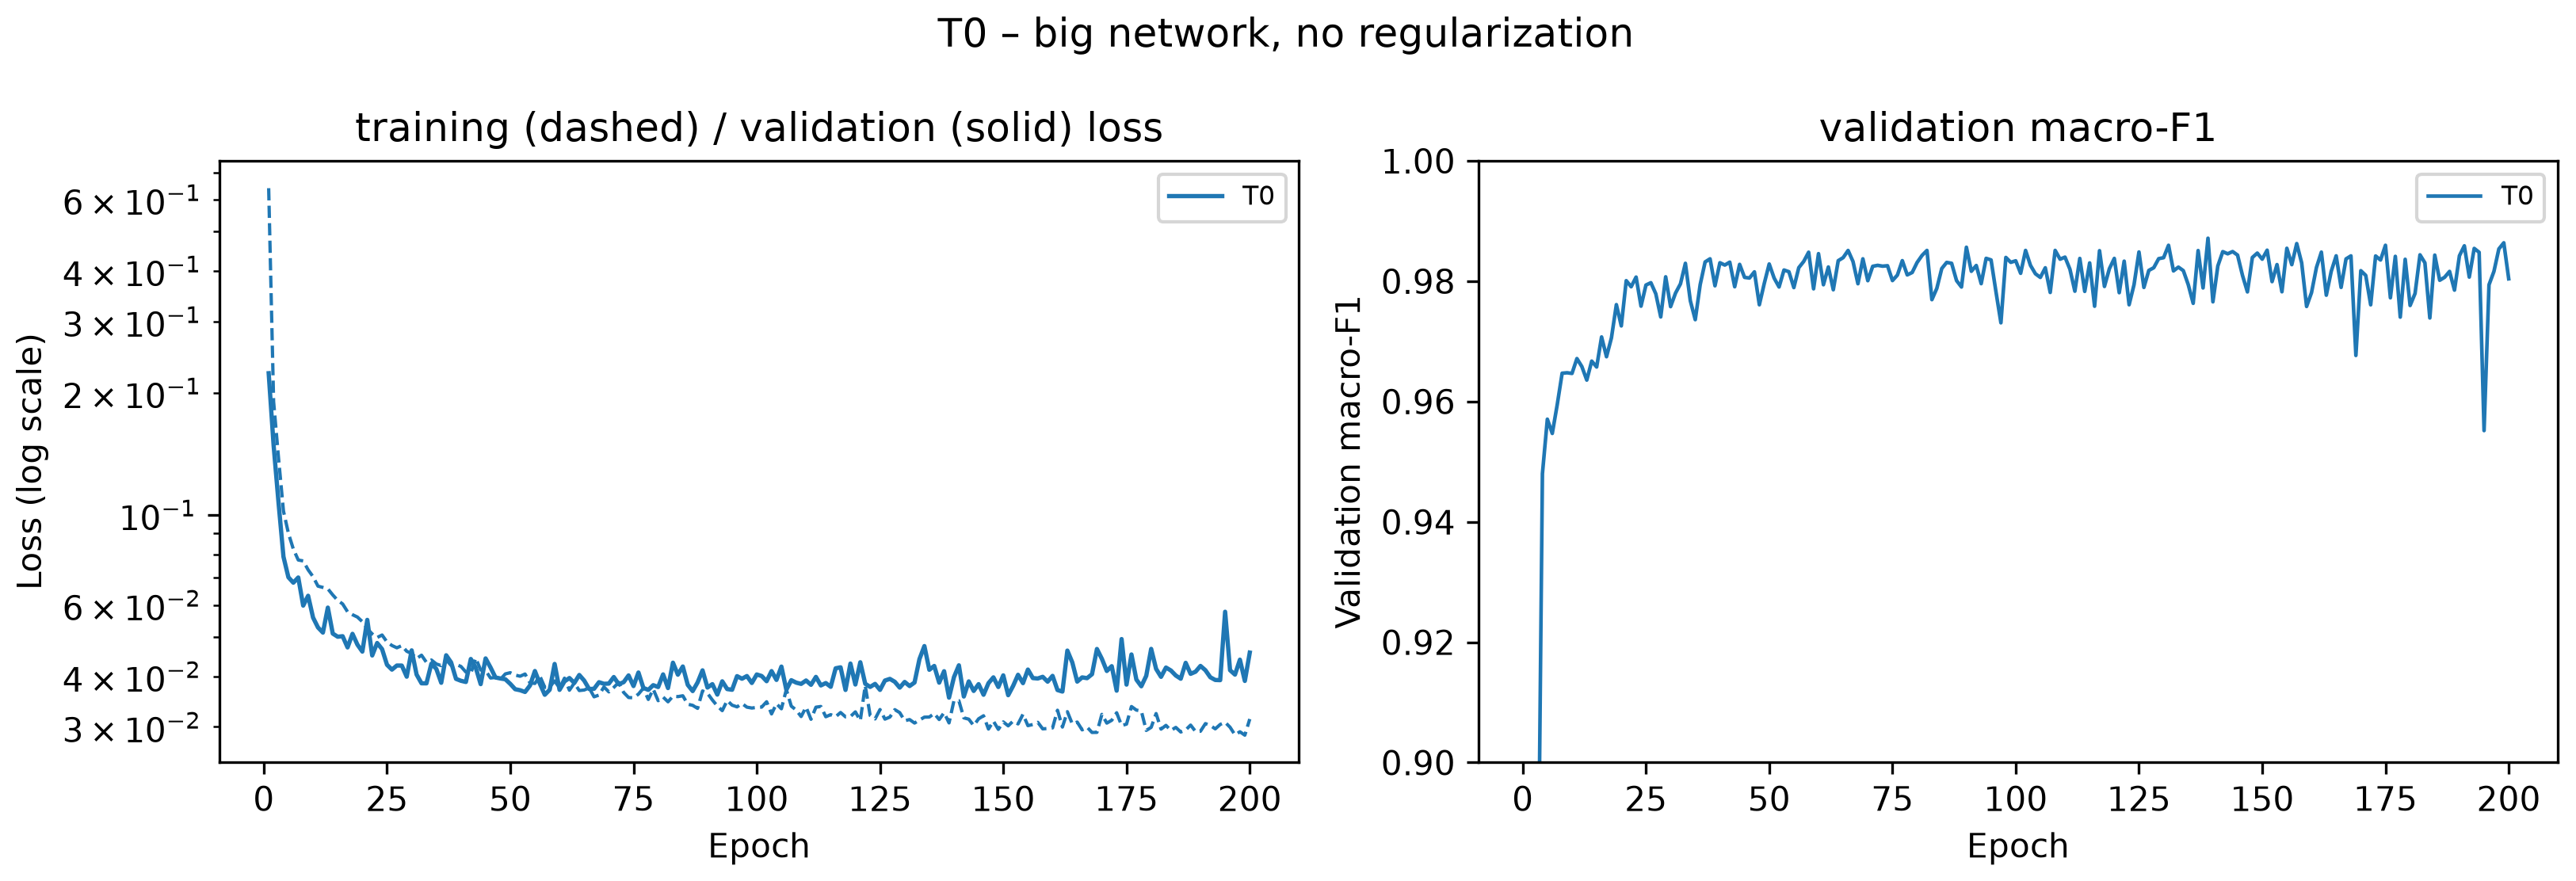
\includegraphics[width=0.82\linewidth]{figures/task6_T0_curves.png}
\caption{\run{T0}. Left: training (dashed) and validation (solid) loss; the curves cross between epochs 60 and 70, the validation minimum is at epoch 139 (0.0354) and the last epoch is at 0.0458. Right: the validation macro-F1 stays on a plateau around 0.98 from epoch 25 on.}
\label{fig:t0}
\end{figure}

\textbf{Prediction (\run{T0}).} A U-shaped validation loss (minimum at epoch 20--60, then rising 1.5--4$\times$), a training loss going towards 0.005--0.02, and val $-$ train turning positive. \emph{Result:} right on the direction, wrong on size and timing. The training loss flattens at about 0.03 (0.0314 at epoch 200): 24,400 updates at lr $5\cdot10^{-4}$ do not memorise the data. The validation loss has no sharp U: it reaches its minimum late (epoch 139) and ends 1.29$\times$ above it.

\Q{Is it overfitting? Show exactly where.} $\rightarrow$ \textbf{Mildly, and mostly in the confidence, not in the decisions.} Three places in Fig.~\ref{fig:t0}: (i) the curves cross between epochs 60 (train 0.0374, val 0.0370) and 70 (0.0366 vs 0.0384), and the validation loss ends clearly above the training loss (+0.0144 at epoch 200; in earlier runs the two stayed within a few thousandths of each other, e.g.\ +0.0023 for \run{P2} at epoch 180 and +0.0009 for \run{D3} at epoch 100); (ii) after its minimum at epoch 139 the validation loss rises to 0.0458 while the training loss keeps falling; (iii) the macro-F1 barely moves (0.9804 at the last epoch, best 0.9871 at epoch 139). The last check explains why: at the last epoch 39 misclassified validation flows (1.2\%) carry 79.0\% of the validation loss, with a median confidence of 0.880 in the wrong class. The loss grows because a few mistakes become very confident, not because the network makes more of them.

\textbf{Plan and rule.} One change per run, simplest first, each checked on validation before the next. Before \run{T2} we fixed the rule: keep a regularizer if, against its parent and at the last epoch, the validation loss falls by at least 10\% and the macro-F1 does not fall by more than 0.01 (the regularizer chain runs without early stopping, so that each regularizer has to fix the overfitting on its own). For step 1 we chose early stopping over a smaller network, because it needs no new hyper-parameter and Task 5 had already measured networks of 1,284--9,604 parameters.

\begin{table}[h]
\centering\footnotesize\setlength{\tabcolsep}{4pt}
\begin{tabular}{llrrrrrl}
\toprule
run & change & macro-F1 & val loss (returned) & min val loss (ep.) & missed / false al. & time (s) & decision \\
\midrule
\run{T0} & prescribed network & 0.9804 & 0.0458 & 0.0354 (139) & 14 / 25 & 60.9 & -- \\
\run{T1 (←T0)} & early stopping & 0.9796 & 0.0384 & 0.0384 (33) & 21 / 16 & 13.8 & 4.4$\times$ cheaper \\
\run{T2 (←T0)} & weight decay 0.1 & 0.9799 & 0.0433 ($-5.5$\%) & 0.0338 (142) & 7 / 29 & 60.0 & dropped \\
\run{T3 (←T0)} & dropout 0.2 & \textbf{0.9849} & 0.0364 ($-20.4$\%) & 0.0317 (103) & 10 / 22 & 75.7 & \textbf{kept} \\
\run{T4 (←T3)} & + batch norm & 0.9842 & 0.0348 ($-4.5$\%) & 0.0328 (132) & 14 / 19 & 98.6 & dropped \\
\bottomrule
\end{tabular}
\caption{Task 6 runs (validation). ``Returned'' is the last epoch, except for \run{T1}, which returns its best epoch. Percentages are against the parent run.}
\label{tab:t6}
\end{table}

\begin{figure}[h]
\centering
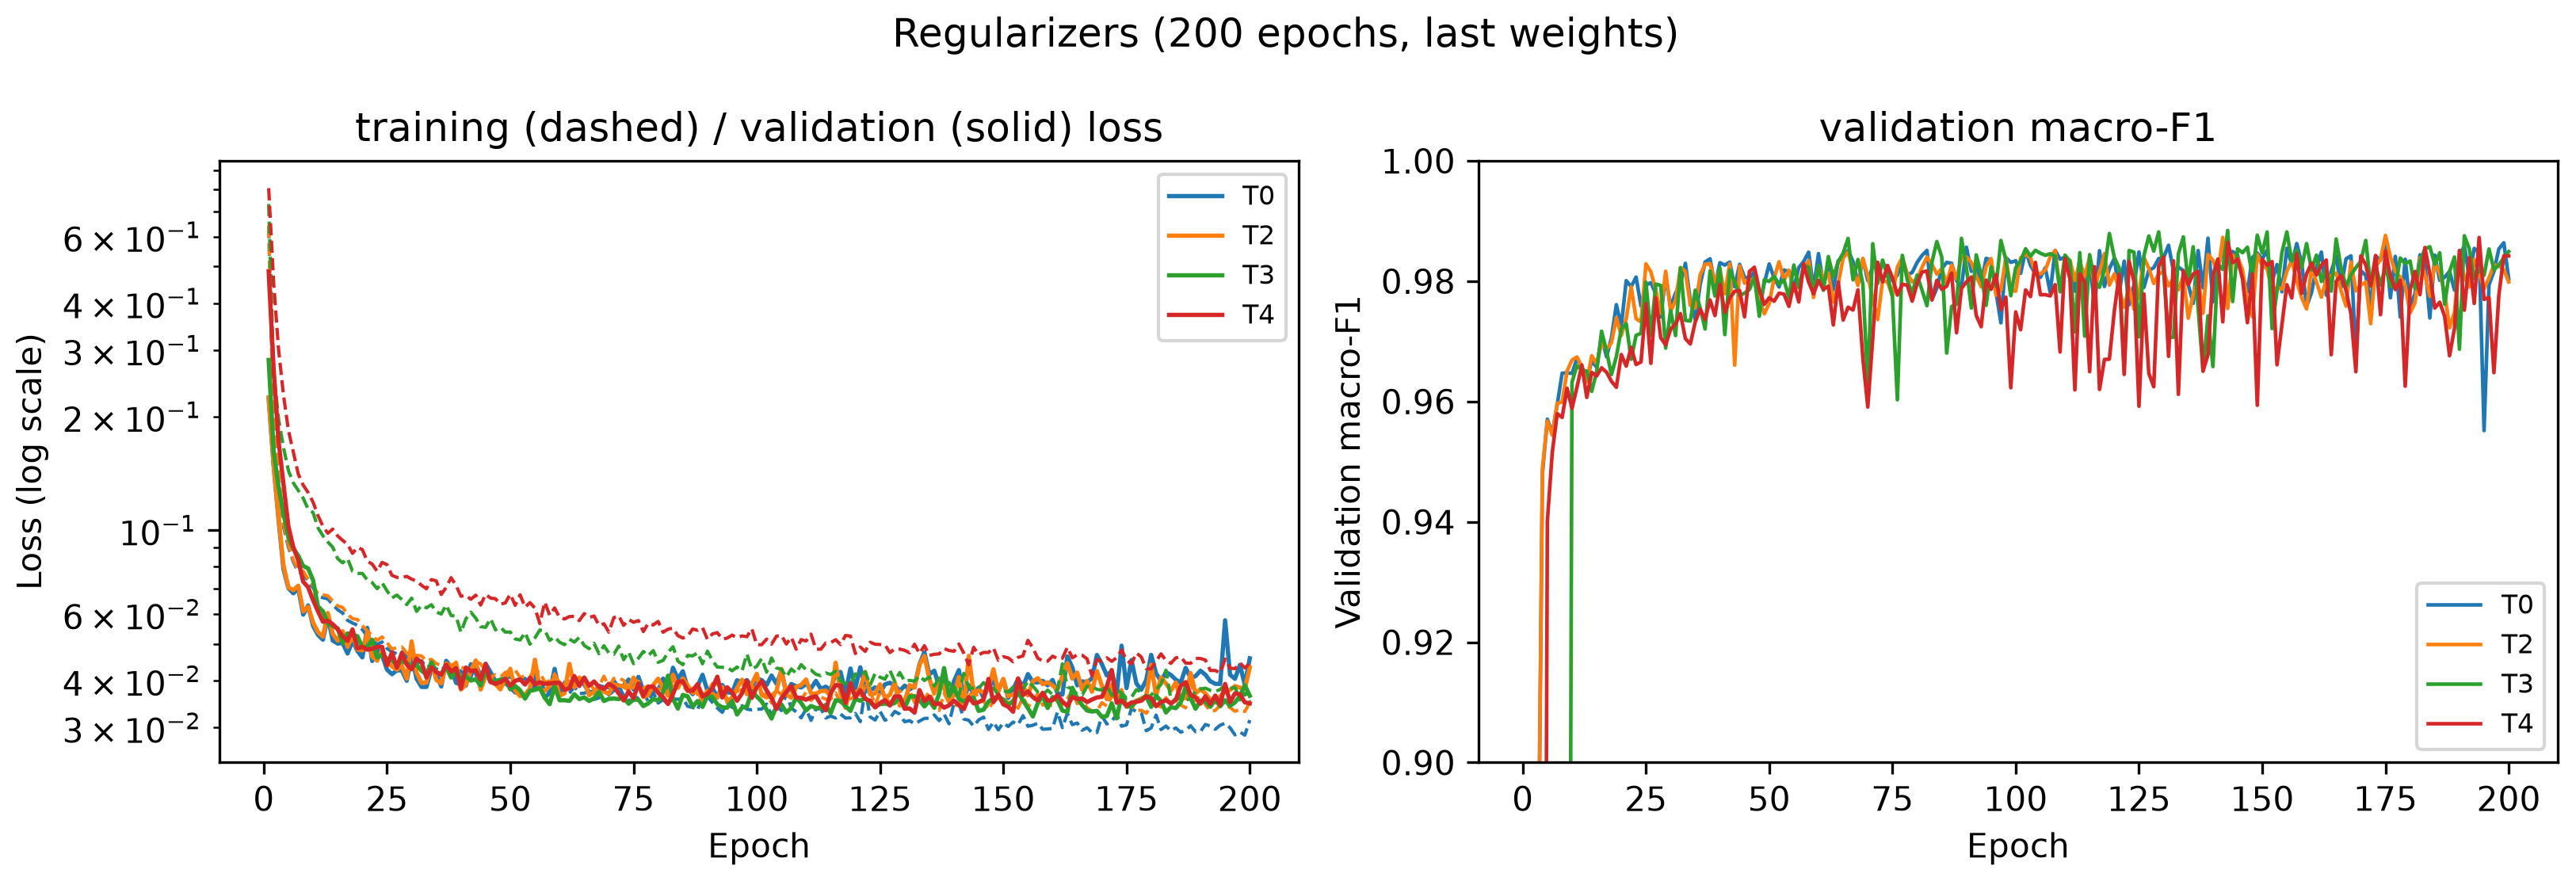
\includegraphics[width=0.7\linewidth]{figures/task6_regularizers_curves.png}
\caption{\run{T0}, \run{T2}, \run{T3} and \run{T4} over 200 epochs (last weights). Left: training (dashed) and validation (solid) loss; with dropout (\run{T3}) and batch norm (\run{T4}) the training loss stays above the validation loss. Right: validation macro-F1; \run{T4} has the deepest dips.}
\label{fig:reg}
\end{figure}

\textbf{What happened.} \run{T1} stopped at epoch 42 on an early plateau and gave the same macro-F1 as \run{T0} in 13.8 s instead of 60.9 s; there was little overfitting to cut. Weight decay (\run{T2}) did much less than predicted ($-5.5$\% against an expected $-20$ to $-50$\%) and was dropped. Dropout (\run{T3}) was the only clear effect (Fig.~\ref{fig:reg}): last-epoch validation loss $-20.4$\%, only 1.15$\times$ its own minimum, the lowest minimum on the port-free data (0.0317) and macro-F1 +0.0045 over \run{T0}. A plausible reading, not tested: a network that cannot rely on single units has a harder time building very confident outputs, which is exactly the mechanism we found in \run{T0}. Batch norm (\run{T4}) on top of dropout gained 4.5\% and was dropped; it also made the curves noisier and was 30\% slower per epoch (0.4928 vs 0.3786 s). Because our rule used a single last-epoch value on curves that move 5--10\% between epochs, we re-checked it on the mean of the last 20 epochs: the decisions do not change ($-9.6$\% for \run{T2}, $-15.9$\% for \run{T3}, $+2.0$\% for \run{T4}), but \run{T2} becomes borderline, and averaging would have been the better rule from the start.

\Q{Which change helped the most for the least effort?} $\rightarrow$ \textbf{Early stopping}: no new hyper-parameter, a flag already in our code, the same detector in under a quarter of the time. \textbf{Dropout} is the only change that clearly improved something, the validation loss, i.e.\ the calibration of the probabilities; its macro-F1 gain is below our 0.01 threshold.

\Q{Did the big network beat the simple port-free baseline on the test set?} $\rightarrow$ \textbf{Against \run{P1}, yes; but not because it is big.} We evaluated the best Task 6 model on validation, \run{T3}, once on the test set. \run{T3} reaches macro-F1 0.9747 against 0.9551 for \run{P1} (10 missed attacks instead of 36; Table~\ref{tab:test5}). But \run{O4}, which has \run{P1}'s architecture, does the same (0.9770) with 37$\times$ fewer parameters and about a fifth of the training time (15.5 vs 75.7 s). The gain over \run{P1} comes from how the network is trained, not from its size. \run{T3} does offer a different trade-off: the fewest missed attacks (10, vs 19 for \run{O4}), thanks to DoS Hulk (test recall 0.986 vs 0.972), at the price of 6 more false alarms (27 vs 21). Whether that is worth it is a deployment question (the cost of a miss vs a false alarm), not a win on our metric. Limit: the port-free test set has now been used for three models (\run{P1}, \run{O4}, \run{T3}), so differences of a few flows should not be read as a ranking.

%==========================================================
\section{Final reflection -- what gave the most per unit of effort}
\begin{table}[h]
\centering\small
\begin{tabular}{p{0.34\linewidth}p{0.08\linewidth}p{0.45\linewidth}}
\toprule
decision & runs & effect (macro-F1 on validation unless stated) \\
\midrule
scale the inputs (\run{S1} vs \run{R1}) & 1 & 0.6943 $\rightarrow$ 0.9365; a whole class lost without it \\
$\log(1+x)$ before scaling (\run{R1} $\rightarrow$ \run{R1L}) & 1 & 0.9365 $\rightarrow$ 0.9875; errors 182 $\rightarrow$ 28 \\
removing the port (Task 3) & 0 & Brute Force test recall 0.995 $\rightarrow$ 0.000 under a port change: the Task 2 scores were not real \\
lr in the right range (\run{S3}; \run{O1} $\rightarrow$ \run{O2}) & 2 & lr 100$\times$ too small: 0.9128 (Adam, data with the port), 0.6975 (SGD); SGD at its own lr 0.9735 \\
epoch cap (\run{R2}) & 1 & +0.0019; converged baseline \\
optimizer + lr (\run{O4}) & 5 & +0.0109 (+0.0219 on test); trains in 15.5 s against 26.6 s for \run{P1} \\
class weights (\run{P2}) & 1 & $-0.0357$; 26 misses traded for 55 false alarms \\
depth (\run{D1}--\run{D3}) and batch size (\run{B1}, \run{B2}) & 5 & at most +0.0095; batch 1 about 14$\times$ the time \\
big network + regularizers (\run{T0}--\run{T4}) & 5 & best 0.9849 (\run{T3}); the same test result as \run{O4} with 37$\times$ the parameters \\
\bottomrule
\end{tabular}
\caption{Decisions across the logbook and what each one bought.}
\label{tab:final}
\end{table}

The decisions that paid most were the \textbf{fundamentals and the data}, not the model (Table~\ref{tab:final}). Scaling and $\log(1+x)$ moved macro-F1 by 0.05--0.3 for one run each, and the most important result of the lab, that the Task 2 model detected port 80 rather than brute force, cost no training run at all, only a counterfactual and a careful look at the duplicates. The learning rate came next: it decided whether SGD worked at all, and the best Task 5 model (\run{O4}) differs from the baseline only in how it is trained. Complexity gave nothing beyond our threshold: depth, batch size, the big network and its regularizers took 10 runs, and none beat the best one-layer network (\run{O4}) by more than 0.01. The remaining errors, mostly DoS Hulk flows that look like Benign in these 15 features, are a property of the data that capacity cannot fix. Two of our 27 runs answered nothing new (\run{S2-lr0.01} and \run{D2}): without them we would have stayed within the budget. If we started again we would measure the seed variance first, to ground our 0.01 threshold, and spend the Task 5 budget on the learning rate rather than on depth.

\clearpage
\appendix
% Appendix A - Experiment logbook (27 runs). Requires in the preamble:
% \usepackage{longtable} \usepackage{array}
\section*{Appendix A -- Experiment logbook}
One row per run that trains a model, in the order of the notebook; the run each one starts from is in brackets and the run name is the Markdown header of its cell (the four S2 runs share the sweep cell). Key result = validation set. Evaluations of already-trained models on the test set (2C, 3.2, 5D, Task 6) are not runs. Budget: Task 2: 10 runs; Task 4: 2; Task 5: 10; Task 6: 5; \textbf{total 27}, two more than the $\sim$25 of the lab text (S2-lr0.01 and D2, redundant in hindsight).

{\footnotesize
\setlength{\tabcolsep}{3pt}
\renewcommand{\arraystretch}{1.15}
\begin{longtable}{>{\raggedright\arraybackslash}p{0.10\linewidth}>{\raggedright\arraybackslash}p{0.035\linewidth}>{\raggedright\arraybackslash}p{0.145\linewidth}>{\raggedright\arraybackslash}p{0.215\linewidth}>{\raggedright\arraybackslash}p{0.225\linewidth}>{\raggedright\arraybackslash}p{0.20\linewidth}}
\hline
\textbf{Run} & \textbf{Task} & \textbf{What I changed (one thing)} & \textbf{Hypothesis before running} & \textbf{Key result (val)} & \textbf{What I concluded} \\ \hline
\endfirsthead
\hline
\textbf{Run} & \textbf{Task} & \textbf{What I changed (one thing)} & \textbf{Hypothesis before running} & \textbf{Key result (val)} & \textbf{What I concluded} \\ \hline
\endhead
R1 & 2A & starting point: 1 hidden layer of 64 ReLU, AdamW lr 5e-4, batch 64, $\leq$100 epochs, patience 10, standard scaling & Brute Force hardest (rarest, inside the bulk), missed as Benign; DoS Hulk and PortScan easiest; macro-F1 $<$ accuracy; early stop before epoch 100 & macro-F1 0.9365, acc. 0.9587; Brute Force precision 0.824 (43 false positives, all Benign on port 80), recall 0.944; lowest recalls PortScan 0.928, DoS Hulk 0.934; best epoch 100/100 (val loss 0.1166) & Brute Force fails by false positives, not misses, and port 80 drives them; DoS Hulk and PortScan lost to Benign; not converged $\rightarrow$ test log1p \\ \hline
R1L ($\leftarrow$R1) & 2A & log1p before the StandardScaler & faster and lower val loss; Brute Force precision $\geq$ 0.85; DoS Hulk and PortScan about unchanged; adopt if macro-F1 +0.01 and no recall $-$0.02 & macro-F1 0.9875 (+0.0510); errors 182 $\rightarrow$ 28; DoS Hulk recall 0.934 $\rightarrow$ 0.993, PortScan 0.928 $\rightarrow$ 0.994; Brute Force precision 0.939; best epoch 99/100 (val loss 0.0273) & log1p kept for the whole lab; the biggest gains came where we expected none: standard scaling had squeezed the DoS Hulk and PortScan features \\ \hline
S1 ($\leftarrow$R1) & 2B & StandardScaler removed (raw inputs, no scaling at all) & start loss 1e3--1e6, jagged curve, no NaN; min val loss far above 0.027; macro-F1 0.5--0.85 & untrained loss 1.373e+06; first-epoch train loss 86142.1984; min val loss 3058.5143; stop at epoch 13 (best 3); macro-F1 0.6943; Brute Force recall 0.000 & badly conditioned inputs (saturated softmax); scaling is the fundamental to fix first \\ \hline
S2-lr0.01 ($\leftarrow$R1L) & 2B & lr 5e-4 $\rightarrow$ 1e-2 & about as good as R1L, maybe noisier & min val loss 0.0251; val roughness 0.1289 (R1L 0.0361); macro-F1 0.9870; stop at epoch 42 (best 32) & as predicted: as good as R1L but noisier; says nothing about where training breaks (redundant in hindsight) \\ \hline
S2-lr0.1 ($\leftarrow$R1L) & 2B & lr 5e-4 $\rightarrow$ 1e-1 & noisy, worse min val loss, still learning & min val loss 0.0621; val roughness 0.723 (R1L 0.0361); macro-F1 0.9767; stop at epoch 17 & as predicted: noisier, not broken \\ \hline
S2 = S2-lr1 ($\leftarrow$R1L) & 2B & lr 5e-4 $\rightarrow$ 1 & broken: spikes, no smooth descent; criterion: min val loss $>$ 0.31 or NaN & first-epoch train loss 4.3650 ($>$ ln 4); val loss 16.5687 at epoch 10; val roughness 1.657; min val loss 0.1393; macro-F1 0.9036 & overshoot; criterion met by no lr, so lr = 1 is S2 by the fallback rule; min val loss hides the breakdown, roughness shows it \\ \hline
S2-lr10 ($\leftarrow$R1L) & 2B & lr 5e-4 $\rightarrow$ 10 & clearly broken & first-epoch train loss 388.1683; val roughness 3.2596; min val loss 0.2775 ($<$ 0.31); macro-F1 0.9111 & broken in shape but not by our criterion: early stopping restores a lucky epoch \\ \hline
S3 ($\leftarrow$R1L) & 2B & lr 5e-4 $\rightarrow$ 5e-6 & smooth, still falling at epoch 100; val loss $\approx$ R1L after one epoch (0.3--0.5); Brute Force lowest recall & val loss 0.2934 at epoch 100 (R1L at epoch 1: 0.3370); best = last epoch; macro-F1 0.9128; lowest recall DoS Hulk 0.807 & underfitting from too slow optimisation; distance estimate right, class prediction wrong \\ \hline
R2 ($\leftarrow$R1L) & 2C & epoch cap 100 $\rightarrow$ 200 & min val loss 0.019--0.0245, best epoch 120--200; macro-F1 +0.000 to +0.005; adopt if val loss $-$10\% and no recall $-$0.01 & min val loss 0.0232 ($-$14.8\%); best epoch 158, stop 168; macro-F1 0.9894 (+0.0019); max recall loss 0.000 & criterion met: R2 replaces R1L as the baseline (converged) \\ \hline
R3 ($\leftarrow$R1L) & 2C & ReLU $\rightarrow$ linear hidden layer (no activation) & min val loss 0.10--0.30; macro-F1 0.85--0.93 (at least $-$0.05); Brute Force precision $<$ 0.80 & min val loss 0.1306; macro-F1 0.9308 ($-$0.0567); Brute Force precision 0.803, recall 0.860; 123 of the 137 errors among Benign / Brute Force / DoS Hulk are on port 80 & ReLU kept; a linear model cannot isolate ``port $\approx$ 80'' \\ \hline
P1 ($\leftarrow$R2) & 4 & data with the port $\rightarrow$ port-free data (15 features) & PortScan suffers most (recall 0.6--0.9); Brute Force recall $\geq$ 0.9, precision 0.8--0.92; accuracy 0.975--0.99, macro-F1 0.90--0.95 & macro-F1 0.9726, acc. 0.9841; PortScan 39 of 42 (recall 0.929, precision 1.000); DoS Hulk recall 0.949 (28 $\rightarrow$ Benign); 31 missed attacks, 20 false alarms; best epoch 92/102 & PortScan still detected; without the port DoS Hulk suffers most; reference for Task 5 \\ \hline
P2 ($\leftarrow$P1) & 4 & unweighted $\rightarrow$ class-weighted cross-entropy (balanced, from the training labels) & accuracy $-$0.001 to $-$0.01, macro-F1 +0.005 to +0.04, PortScan recall $\geq$ 0.95; wrong if macro-F1 falls & macro-F1 0.9369 ($-$0.0357); acc. 0.9751; macro-recall 0.9663 $\rightarrow$ 0.9883; missed attacks 31 $\rightarrow$ 5, false alarms 20 $\rightarrow$ 75; PortScan precision 0.750 & the ``wrong if'' happened: P1 was not under-detecting; the weights trade 26 misses for 55 false alarms; P1 kept \\ \hline
D1 ($\leftarrow$P1) & 5A & hidden layers [64] $\rightarrow$ [64, 64] & depth does not help: macro-F1 within $\pm$0.01 of P1; earlier best epoch & macro-F1 0.9820 (+0.0094); DoS Hulk recall 0.9495 $\rightarrow$ 0.9739; best epoch 61 & gain below threshold (about three PortScan flows); faster convergence \\ \hline
D2 ($\leftarrow$P1) & 5A & [64] $\rightarrow$ [64, 64, 64] (9,604 params) & as D1; gap less negative, maybe slightly positive & macro-F1 0.9821 (+0.0095); best epoch 40; gap $-$0.0017 & a third layer adds nothing over the second; no overfitting (redundant in hindsight) \\ \hline
D3 ($\leftarrow$P1) & 5A & [64] $\rightarrow$ [32, 32] (1,700 params) & behaves like P1 & macro-F1 0.9750 (+0.0024); best epoch 92, as P1 & depth at constant parameter count changes nothing \\ \hline
B1 ($\leftarrow$P1) & 5B & batch 64 $\rightarrow$ 1 & jagged curve, best epoch $\leq$15, macro-F1 P1 $-$0.02 to +0.005; time $\times$5--15 & macro-F1 0.9706 ($-$0.0020); best epoch 37; 360.4 s (P1: 26.6 s) & no gain at about 14$\times$ the time; val roughness 3$\times$ P1 (0.0926 vs 0.0307); best epoch later than predicted \\ \hline
B2 ($\leftarrow$P1) & 5B & batch 64 $\rightarrow$ 1024 & underfits (3,200 updates), macro-F1 $-$0.02 to $-$0.08; 3--6$\times$ faster & macro-F1 0.9567 ($-$0.0159); best epoch 199/200; 27.1 s (P1: 26.6 s) & underfitting from too few updates; not faster in total (wrong on time) \\ \hline
O1 ($\leftarrow$P1) & 5C & AdamW $\rightarrow$ SGD (lr 5e-4) & far too slow; macro-F1 0.6--0.9; PortScan $\sim$0 & macro-F1 0.6975; PortScan recall 0.000; best epoch 200/200 (still falling) & SGD needs a much larger lr than Adam \\ \hline
O2 ($\leftarrow$O1) & 5C & lr 5e-4 $\rightarrow$ 5e-2 (SGD) & within 0.02 of P1 & macro-F1 0.9735 (+0.0010) & at its own lr SGD matches AdamW \\ \hline
O3 ($\leftarrow$O1) & 5C & + momentum 0.9 (SGD, lr 5e-4) & $\sim$10$\times$ faster than O1, not converged; macro-F1 0.85--0.95 & macro-F1 0.9521; best epoch 200/200 (still falling) & momentum helps, but the lr is still too small \\ \hline
O4 ($\leftarrow$O3) & 5C & lr 5e-4 $\rightarrow$ 5e-2 (SGD + momentum 0.9) & close to P1, roughest SGD curve, stops earliest & macro-F1 0.9835 (+0.0109); missed attacks 31 $\rightarrow$ 16; stop at 76 & best run of Task 5; meets the criterion by 0.0009 (wrong prediction) $\rightarrow$ replaces P1 as reference \\ \hline
O5 ($\leftarrow$P1) & 5C & AdamW lr 5e-4 $\rightarrow$ 5e-2 & jagged, early stop $<$ 60, macro-F1 $-$0.03 to 0 & macro-F1 0.9665 ($-$0.0061); best epoch 5; val roughness 0.2996 (P1: 0.0307) & Adam tolerates a 100$\times$ lr range; lr dominates for SGD, not for AdamW \\ \hline
T0 & 6 & new starting point set by the lab text (not a one-change run): big network, weight decay 0, no early stopping & U-shaped val loss (min at ep. 20--60, ends 1.5--4$\times$ higher); train loss $\rightarrow$ 0.005--0.02; macro-F1 0.96--0.98 & min val loss 0.0354 (epoch 139) $\rightarrow$ 0.0458 at epoch 200 ($\times$1.29); train loss 0.0314; val $-$ train +0.0144; macro-F1 0.9804 & mild overfitting, mostly in the confidence (39 mistakes = 79.0\% of the loss); macro-F1 barely affected \\ \hline
T1 ($\leftarrow$T0) & 6 & early stopping (patience 10) & stop at ep. 30--70; better than T0 last epoch by 0.005--0.02; 3--6$\times$ faster & stop at 42 (best 32); macro-F1 0.9796; 13.8 s vs 60.9 s & same detector at under 1/4 of the cost; stopped on an early plateau \\ \hline
T2 ($\leftarrow$T0) & 6 & weight decay 0 $\rightarrow$ 0.1 & last-epoch val loss $-$20 to $-$50\%; macro-F1 $\pm$0.01; kept & val loss 0.0458 $\rightarrow$ 0.0433 ($-$5.5\%); macro-F1 0.9799; 7 missed / 29 false alarms & dropped by the rule (borderline once averaged: $-$9.6\%) \\ \hline
T3 ($\leftarrow$T0) & 6 & + dropout 0.2 & train $>$ val; val loss $\leq$1.3$\times$ its min, $-$10\% or more; macro-F1 $\pm$0.01; kept & val loss 0.0458 $\rightarrow$ 0.0364 ($-$20.4\%), $\times$1.15 its min; macro-F1 0.9849 & kept; the only regularizer with a clear effect (on the loss) \\ \hline
T4 ($\leftarrow$T3) & 6 & + batch norm & faster start; val loss not $-$10\%; noisier; dropped & val loss 0.0364 $\rightarrow$ 0.0348 ($-$4.5\%; +2.0\% averaged); macro-F1 0.9842 ($-$0.0007); slower start; noisier curves & dropped; no gain, s/epoch 0.4928 vs 0.3786 (+30\%), noisier than T3 \\ \hline
\end{longtable}
}


\end{document}
